% The main file. It contains definitions of basic 
% parameters and includes all other parts.

%% Settings for single-side (simplex) printing
% Margins: left 40mm, right 25mm, top and bottom 25mm
% (but beware, LaTeX adds 1in implicitly)
\documentclass[12pt,a4paper]{report}
\setlength\textwidth{145mm}
\setlength\textheight{247mm}
\setlength\oddsidemargin{15mm}
\setlength\evensidemargin{15mm}
\setlength\topmargin{0mm}
\setlength\headsep{0mm}
\setlength\headheight{0mm}
% \openright makes the following text appear on a right-hand page
\let\openright=\clearpage 

%% Settings for two-sided (duplex) printing
% \documentclass[12pt,a4paper,twoside,openright]{report}
% \setlength\textwidth{145mm}
% \setlength\textheight{247mm}
% \setlength\oddsidemargin{14.2mm}
% \setlength\evensidemargin{0mm}
% \setlength\topmargin{0mm}
% \setlength\headsep{0mm}
% \setlength\headheight{0mm}
% \let\openright=\cleardoublepage

%% Generate PDF/A-2u
\usepackage[a-2u]{pdfx}

%% Character encoding: usually latin2, cp1250 or utf8:
\usepackage[utf8]{inputenc}

%% Prefer Latin Modern fonts
\usepackage{lmodern}

%% Further useful packages (included in most LaTeX distributions)
\usepackage{amsmath}        % extensions for typesetting of math
\usepackage{amsfonts}       % math fonts
\usepackage{amsthm}         % theorems, definitions, etc.
\usepackage{bbding}         % various symbols (squares, asterisks, scissors, ...)
\usepackage{bm}             % boldface symbols (\bm)
\usepackage{graphicx}       % embedding of pictures
\graphicspath{{img/}}
\usepackage{fancyvrb}       % improved verbatim environment
\usepackage{natbib}         % citation style AUTHOR (YEAR), or AUTHOR [NUMBER]
\usepackage[nottoc]{tocbibind} % makes sure that bibliography and the lists
			    % of figures/tables are included in the table
			    % of contents
\usepackage{dcolumn}        % improved alignment of table columns
\usepackage{booktabs}       % improved horizontal lines in tables
\usepackage{paralist}       % improved enumerate and itemize
\usepackage{xspace}
\usepackage{xcolor}
\usepackage{soul}
% \usepackage[usenames]{xcolor}  % typesetting in color

\usepackage[acronym,toc]{glossaries} % making glossaries

\usepackage[normalem]{ulem} % tables


%%JaKl comment macros - to be removed when cleaning the thesis
\newcommand{\TODO}[1]{{\color{red}{\textbf{TODO: {#1}}\xspace}}}
\newcommand{\CONSIDER}[1]{{\color{blue}{\textbf{CONSIDER: {#1}}\xspace}}}
%%End of JaKl comment macros

%%% Basic information on the thesis

% Thesis title in English (exactly as in the formal assignment)
\def\ThesisTitle{Decentralized Web-based Data Storage for LinkedPipes Applications using Solid}

% Author of the thesis
\def\ThesisAuthor{Altynbek Orumbayev}

% Year when the thesis is submitted
\def\YearSubmitted{2019}

% Name of the department or institute, where the work was officially assigned
% (according to the Organizational Structure of MFF UK in English,
% or a full name of a department outside MFF)
\def\Department{Department of Software Engineering}

% Is it a department (katedra), or an institute (ústav)?
\def\DeptType{Department}

% Thesis supervisor: name, surname and titles
\def\Supervisor{RNDr. Jakub Klímek, Ph.D.}

% Supervisor's department (again according to Organizational structure of MFF)
\def\SupervisorsDepartment{department}

% Study programme and specialization
\def\StudyProgramme{Computer Science}
\def\StudyBranch{Software and Data Engineering}

% An optional dedication: you can thank whomever you wish (your supervisor,
% consultant, a person who lent the software, etc.)
\def\Dedication{%
Dedication.
}

% Abstract (recommended length around 80-200 words; this is not a copy of your thesis assignment!)
\def\Abstract{%
Abstract.
}

% 3 to 5 keywords (recommended), each enclosed in curly braces
\def\Keywords{%
{solid, linked data, client, server, storage, web}
}

%% The hyperref package for clickable links in PDF and also for storing
%% metadata to PDF (including the table of contents).
%% Most settings are pre-set by the pdfx package.
\hypersetup{unicode}
\hypersetup{breaklinks=true}

% Definitions of macros (see description inside)
%%% This file contains definitions of various useful macros and environments %%%
%%% Please add more macros here instead of cluttering other files with them. %%%

%%% Minor tweaks of style

% These macros employ a little dirty trick to convince LaTeX to typeset
% chapter headings sanely, without lots of empty space above them.
% Feel free to ignore.
\makeatletter
\def\@makechapterhead#1{
  {\parindent \z@ \raggedright \normalfont
   \Huge\bfseries \thechapter. #1
   \par\nobreak
   \vskip 20\p@
}}
\def\@makeschapterhead#1{
  {\parindent \z@ \raggedright \normalfont
   \Huge\bfseries #1
   \par\nobreak
   \vskip 20\p@
}}
\makeatother

% This macro defines a chapter, which is not numbered, but is included
% in the table of contents.
\def\chapwithtoc#1{
\chapter*{#1}
\addcontentsline{toc}{chapter}{#1}
}

% Draw black "slugs" whenever a line overflows, so that we can spot it easily.
\overfullrule=1mm

%%% Macros for definitions, theorems, claims, examples, ... (requires amsthm package)

\theoremstyle{plain}
\newtheorem{thm}{Theorem}
\newtheorem{lemma}[thm]{Lemma}
\newtheorem{claim}[thm]{Claim}

\theoremstyle{plain}
\newtheorem{defn}{Definition}

\theoremstyle{remark}
\newtheorem*{cor}{Corollary}
\newtheorem*{rem}{Remark}
\newtheorem*{example}{Example}

%%% An environment for proofs

%%% FIXME %%% \newenvironment{proof}{
%%% FIXME %%%   \par\medskip\noindent
%%% FIXME %%%   \textit{Proof}.
%%% FIXME %%% }{
%%% FIXME %%% \newline
%%% FIXME %%% \rightline{$\square$}  % or \SquareCastShadowBottomRight from bbding package
%%% FIXME %%% }

%%% An environment for typesetting of program code and input/output
%%% of programs. (Requires the fancyvrb package -- fancy verbatim.)

\DefineVerbatimEnvironment{code}{Verbatim}{fontsize=\small, frame=single}

%%% The field of all real and natural numbers
\newcommand{\R}{\mathbb{R}}
\newcommand{\N}{\mathbb{N}}

%%% Useful operators for statistics and probability
\DeclareMathOperator{\pr}{\textsf{P}}
\DeclareMathOperator{\E}{\textsf{E}\,}
\DeclareMathOperator{\var}{\textrm{var}}
\DeclareMathOperator{\sd}{\textrm{sd}}

%%% Transposition of a vector/matrix
\newcommand{\T}[1]{#1^\top}

%%% Various math goodies
\newcommand{\goto}{\rightarrow}
\newcommand{\gotop}{\stackrel{P}{\longrightarrow}}
\newcommand{\maon}[1]{o(n^{#1})}
\newcommand{\abs}[1]{\left|{#1}\right|}
\newcommand{\dint}{\int_0^\tau\!\!\int_0^\tau}
\newcommand{\isqr}[1]{\frac{1}{\sqrt{#1}}}

%%% Various table goodies
\newcommand{\pulrad}[1]{\raisebox{1.5ex}[0pt]{#1}}
\newcommand{\mc}[1]{\multicolumn{1}{c}{#1}}

%%% Glossary macros 
\newcommand{\solid}{SOLID}
\newcommand{\lpa}{LinkedPipes Applications Storage}
\newcommand{\lpas}{LinkedPipes Applications Storage}


%% Load glossary
% % Acronyms 
\newacronym{API}{API}{Application Programming Interface}
\newacronym{ETL}{ETL}{Extract, Transform and Load}
\newacronym{IRI}{IRI}{Internationalized Resource Identifier}
\newacronym{URI}{URI}{Uniform Resource Identifier}
\newacronym{URL}{URL}{Uniform Resource Locator}
\newacronym{LPA}{LPA}{LinkedPipes Application}
\newacronym{RDF}{RDF}{ Resource Description Framework}
\newacronym{SPA}{SPA}{Single-page Application}
\newacronym{LDVM}{LDVM}{Linked Data Visualization Model}
\newacronym{LDMVi}{LDVMi}{Linked Data Visualization Model implementation}
\newacronym{TTL}{TTL}{Turtle (syntax)}
\newacronym{LODC}{LOD Cloud}{Linked Open Data Cloud}
\newacronym{SPARQL}{SPARQL}{SPARQL Protocol and RDF Query Language}
\newacronym{W3C}{W3C}{World Wide Web Consortium}
\newacronym{LOV}{LOV}{Linked Open Vocabularies}
\newacronym{DOM}{DOM}{Document Object Model}
\newacronym{SSL}{SSL}{Secure Sockets Layer }
\newacronym{TLS}{TLS}{Transport Layer Security}

% Terms/Definitions
\newglossaryentry{endpoint}
{
    name=Endpoint,
    description={An endpoint is one end of a communication channel}
}

\newglossaryentry{assistant}
{
    name=Assistant,
    description={Refers to the Linked Pipes Visualization Assistant, which allows users to create, configure and publish visualizations based on input data sets}
}

\newglossaryentry{datacube}
{
    name={Data cube},
    description={multi-dimensional array of values}
}

\newglossaryentry{data-descriptor}
{
    name={Data descriptor},
    description={An SPARQL ASK query associated with a visualizer that determines if an input data graph can be visualized in the corresponding visualizer}
}

\newglossaryentry{data-source}
{
    name={Data source},
    description={Refers to any source of data, such as an RDF file, CSV, database, etc}
 }

\newglossaryentry{linked-data}
{
    name={Linked Data},
    description={a method of publishing structured data so that it can be interlinked}
}

\newglossaryentry{lod-cloud}{
    name={Linked Open Data Cloud},
    description={The largest cloud of linked data that is freely available to everyone}
}

\newglossaryentry{lp-etl}
{
    name={LinkedPipes ETL},
    description={The service in charge of the ETL process in the LinkedPipes ecosystem}
}

\newglossaryentry{lp-solid}
{
    name={SOLID},
    description={to write}
}
    
\newglossaryentry{lp-discovery}
{
    name={LinkedPipes Discovery},
    description={The service of the LinkedPipes ecosystem in charge of the process of discovering pipelines to be executed in a particular dataset.}
}

\newglossaryentry{pipeline}
{
    name=Pipeline,
    description={in the current context refers to the process in which the application takes any data source, applies a series of transformations to it and then hands over the output to a visualizer component, which then produces a visual representation of the data}
}

\newglossaryentry{pipeline-disc}
{
    name={pipeline discovery},
    description={The process taking input descriptors for all visualizers and attempt to combine the respective transformation registered to achieve a specific data format}
}

\newglossaryentry{semantic-web}
{
    name={Semantic web},
    description={an extension of the World Wide Web through standards by the World Wide Web Consortium}
}

\newglossaryentry{sparql-def}
{
    name={SPARQL Protocol and RDF Query Language},
    description={query language for retrieving and manipulating data stored in RDF format}
}

% Acronyms 
\newacronym{API}{API}{Application Programming Interface}
\newacronym{ETL}{ETL}{Extract, Transform and Load}
\newacronym{IRI}{IRI}{Internationalized Resource Identifier}
\newacronym{URI}{URI}{Uniform Resource Identifier}
\newacronym{URL}{URL}{Uniform Resource Locator}
\newacronym{LPA}{LPA}{LinkedPipes Application}
\newacronym{RDF}{RDF}{ Resource Description Framework}
\newacronym{SPA}{SPA}{Single-page Application}
\newacronym{LDVM}{LDVM}{Linked Data Visualization Model}
\newacronym{LDMVi}{LDVMi}{Linked Data Visualization Model implementation}
\newacronym{TTL}{TTL}{Turtle (syntax)}
\newacronym{LODC}{LOD Cloud}{Linked Open Data Cloud}
\newacronym{SPARQL}{SPARQL}{SPARQL Protocol and RDF Query Language}
\newacronym{W3C}{W3C}{World Wide Web Consortium}
\newacronym{LOV}{LOV}{Linked Open Vocabularies}
\newacronym{DOM}{DOM}{Document Object Model}
\newacronym{SSL}{SSL}{Secure Sockets Layer }
\newacronym{TLS}{TLS}{Transport Layer Security}

% Terms/Definitions
\newglossaryentry{endpoint}
{
    name=Endpoint,
    description={An endpoint is one end of a communication channel}
}

\newglossaryentry{assistant}
{
    name=Assistant,
    description={Refers to the Linked Pipes Visualization Assistant, which allows users to create, configure and publish visualizations based on input data sets}
}

\newglossaryentry{datacube}
{
    name={Data cube},
    description={multi-dimensional array of values}
}

\newglossaryentry{data-descriptor}
{
    name={Data descriptor},
    description={An SPARQL ASK query associated with a visualizer that determines if an input data graph can be visualized in the corresponding visualizer}
}

\newglossaryentry{data-source}
{
    name={Data source},
    description={Refers to any source of data, such as an RDF file, CSV, database, etc}
 }

\newglossaryentry{linked-data}
{
    name={Linked Data},
    description={a method of publishing structured data so that it can be interlinked}
}

\newglossaryentry{lod-cloud}{
    name={Linked Open Data Cloud},
    description={The largest cloud of linked data that is freely available to everyone}
}

\newglossaryentry{lp-etl}
{
    name={LinkedPipes ETL},
    description={The service in charge of the ETL process in the LinkedPipes ecosystem}
}

\newglossaryentry{lp-solid}
{
    name={SOLID},
    description={to write}
}
    
\newglossaryentry{lp-discovery}
{
    name={LinkedPipes Discovery},
    description={The service of the LinkedPipes ecosystem in charge of the process of discovering pipelines to be executed in a particular dataset.}
}

\newglossaryentry{pipeline}
{
    name=Pipeline,
    description={in the current context refers to the process in which the application takes any data source, applies a series of transformations to it and then hands over the output to a visualizer component, which then produces a visual representation of the data}
}

\newglossaryentry{pipeline-disc}
{
    name={pipeline discovery},
    description={The process taking input descriptors for all visualizers and attempt to combine the respective transformation registered to achieve a specific data format}
}

\newglossaryentry{semantic-web}
{
    name={Semantic web},
    description={an extension of the World Wide Web through standards by the World Wide Web Consortium}
}

\newglossaryentry{sparql-def}
{
    name={SPARQL Protocol and RDF Query Language},
    description={query language for retrieving and manipulating data stored in RDF format}
}


% \makeglossaries
\makenoidxglossaries

% Title page and various mandatory informational pages
\begin{document}
%%% Title page of the thesis and other mandatory pages

%%% Title page of the thesis

\pagestyle{empty}
\hypersetup{pageanchor=false}
\begin{center}

\centerline{\mbox{
\includegraphics[width=166mm]{img/logo-en.pdf}}}

\vspace{-8mm}
\vfill

{\bf\Large MASTER THESIS}

\vfill

{\LARGE\ThesisAuthor}

\vspace{15mm}

{\LARGE\bfseries\ThesisTitle}

\vfill

\Department

\vfill

\begin{tabular}{rl}

Supervisor of the master thesis: & \Supervisor \\
\noalign{\vspace{2mm}}
Study programme: & \StudyProgramme \\
\noalign{\vspace{2mm}}
Study branch: & \StudyBranch \\
\end{tabular}

\vfill

% Zde doplňte rok
Prague \YearSubmitted

\end{center}

\newpage

%%% Here should be a bound sheet included -- a signed copy of the "master
%%% thesis assignment". This assignment is NOT a part of the electronic
%%% version of the thesis. DO NOT SCAN.

%%% A page with a solemn declaration to the master thesis

\openright
\hypersetup{pageanchor=true}
\pagestyle{plain}
\pagenumbering{roman}
\vglue 0pt plus 1fill

\noindent
I declare that I carried out this master thesis independently, and only with the cited
sources, literature and other professional sources.

\medskip\noindent
I understand that my work relates to the rights and obligations under the Act No.~121/2000 Sb.,
the Copyright Act, as amended, in particular the fact that the Charles
University has the right to conclude a license agreement on the use of this
work as a school work pursuant to Section 60 subsection 1 of the Copyright Act.

\vspace{10mm}

\hbox{\hbox to 0.5\hsize{%
In ........ date ............	% FIXME!
\hss}\hbox to 0.5\hsize{%
signature of the author
\hss}}

\vspace{20mm}
\newpage

%%% Dedication

\openright

\noindent
\Dedication

\newpage

%%% Mandatory information page of the thesis

\openright

\vbox to 0.5\vsize{
\setlength\parindent{0mm}
\setlength\parskip{5mm}

Title:
\ThesisTitle

Author:
\ThesisAuthor

\DeptType:
\Department

Supervisor:
\Supervisor, \SupervisorsDepartment

Abstract:
\Abstract

Keywords:
\Keywords

\vss}

\newpage

\openright
\pagestyle{plain}
\pagenumbering{arabic}
\setcounter{page}{1}


%%% A page with automatically generated table of contents of the master thesis

\tableofcontents

%%% Each chapter is kept in a separate file
\chapter*{Introduction}
\label{chap:introduction}
% \addcontentsline{toc}{chapter}{Introduction}

The World Wide Web as we know it started on March 12, 1989, by Sir Tim Berners-Lee. What began as a proposal, eventually ended up being one of the most important technological achievements of a century. Nowadays, the ability to access information online is often an effortless process. People can easily use a search engine to look up articles, connect with anyone in a matter of seconds using social network platforms, consume gigabytes of media \cite{www_foundation_intro}. Furthermore, most importantly \TODO{just one of furthermore and most importantly}, they can upload, store, and share any data online. When it comes to storing data online, an average \TODO{Internet, (capital I) when you mean the global one} internet user will most probably rely on companies providing their storage solutions in the \textit{Cloud}. The majority of popular cloud storage providers like \textit{Google}, \textit{Dropbox} or \textit{Microsoft OneDrive} are centralized. Centralization is in no means a matter of a concern for an average internet user.

On the contrary, it usually provides a better user experience when the user has all of his relevant data stored in a centralized \textit{data silo}. The term \textit{data silo} often describes a fixed repository of data entirely under control of a single department while being isolated from the rest of the organization. On the other hand, it raises a lot of privacy concerns when it comes to explaining who owns the data stored under such cloud storage. With the growth of large software corporations and an increase in the dominance of their services and technologies where billions of users upload, store and share data under their centralized silos, a lot of examples of disadvantages of centralization were demonstrated for the past several years. For example, an infamous \textit{Facebook–Cambridge Analytica} data scandal in early 2018 \footnote{\url{https://en.wikipedia.org/wiki/Facebook–Cambridge_Analytica_data_scandal}}, demonstrated how millions of \textit{Facebook} profiles were analyzed without any consent and later targeted for political advertising. In a certain sense, the fact that data was under control of a single organization and stored in centralized fashion played an important role in raising privacy concerns and making people more cautious about relying on centralized providers to own their data.

On August 10, 2016, another ambitious project was launched by Sir Tim Berners-Lee called \solid{} \footnote{\url{https://solidproject.org}}. The goal of the project is to make World Wide Web decentralized, improve data ownership on the internet, and give the full control over the data back to the users by providing an alternative to dominating storage technologies relying on centralized data silos. Even though the idea might be appealed as too ambitious, over the years, the project has grown from several proof-of-concept proposals to a large community of developers actively contributing and expanding the project every day. The \solid{} project, by definition, represents multiple things at once. In formal terms, it is a set of specifications, principles, conventions, and tools for building \textit{decentralized social applications} while relying on principles of \textit{Linked Data}. The term \solid{} by itself stands for \textit{Social Linked Data}, where the term \textit{Linked Data} stands for yet another concept that will be heavily utilized in this thesis project. Linked Data is a method for publishing structured data in a way that preserves the semantics of the data. This semantic description is implemented by the use of \textit{vocabularies} \footnote{\url{https://www.w3.org/standards/semanticweb/ontology}}, which are usually specified by the \acrshort{W3C} as web standards. However, anyone can create and register their vocabulary, for example, in an open catalog like \textit{\gls{LOV}} \footnote{\url{https://lov.linkeddata.es/dataset/lov/}}. Linked data is usually dispersed across many sites on the internet. Each site usually contains only a part of the entire data available. Thus a machine or a person trying to interpret the data as a whole needs to link this incomplete information together using unique entity identifiers shared across the data stores. Another common term usually associated with Linked Data is \textit{Linked Open Data}, in contrast with Linked Data, it follows the \textit{five star Linked Open Data} model \footnote{\url{https://www.w3.org/community/webize/2014/01/17/what-is-5-star-linked-data/}}. It represents Linked Data that is publicly accessible to everyone.

In November 2018, a group of five Master students, including the myself, at Faculty of Mathematics and Physics at Charles Univesity in Prague, started a university software project called \textit{\gls{LPA}}. The project was focused around development of a web app that would simplify the interactions with Linked Data and other concepts of \textit{Semantic Web} \footnote{\url{https://www.w3.org/standards/semanticweb/}} for average \textit{lay} users and provide an intuitive and straightforward way to visualize Linked Data expressed in \textit{RDF} format for various needs. The initial goals of that project did not involve any plans to rely on any decentralized storages, such as ones represented by \solid{}. However, over time the set of functional and non-functional requirements related to dealing with massive amounts of Linked Data expressed in RDF format, ability to share the applications created with the platform while maintaining the control over them, and most importantly storing and sharing the \lpa{} platform data became specific enough to become a perfect fit to use \solid{} as a primary technology for storing the data. 
 
\section*{Goal of the thesis}
% Solid mentions
The main goal of the following thesis is to provide a decentralized web-based storage solution based on \solid{} project for the \lpa{} platform and demonstrate the full benefits of decentralized storage and the \solid{} technology. The results of the practical work must satisfy all defined functional and non-functional requirements stated by \lpa{} project. The complete implementation of the solution implementing the requirements must be provided and described in detail as a part of this thesis. It is important to note that the \solid{} project is still in the early stages of development, and its specifications are being updated regularly. Therefore, aside from fitting the needs of \lpa{} requirements, the implemented toolset must be generic enough for the possibility to be extended for usage in any application using \solid{}. Further mentions of the practical part of this thesis are going to be called as \textit{\gls{LPS}}.

\section*{Structure}

The structure consist of nine main chapters that can be described as follows:
\begin{enumerate}
    \item \textit{Preliminaries}, Basic introduction to core concepts of \textit{Semantic Web} and \solid{} that will be appearing throughout the rest of the thesis. The remaining sections of the chapter are dedicated to general description and main concepts of \lpa{}. That project defines the core requirements for this thesis, therefore it is important to make sure that all \lpa{} specific terms and definitions are explained before proceeding to further chapters.
    
    \item \textit{Overview of decentralized web-based storage technologies}, the chapter provides an overview of decentralized software technologies that are alternative or opposed to concepts of \solid{}. Additionally, the chapter also provides the core ideas on why \solid{} turned out to be a perfect fit for \lpa{}.

    \item \textit{Analysis}, chapter is an overview of all functional and non-functional requirements stated by \lpa{} as they are the main users of the \lpas{}.

    \item \textit{Architecture}, chapter continues the \textit{Analysis} chapter by describing the architecture of the solution. Additionally, the first section of the chapter provides a review of technologies, frameworks, and libraries that were under assumption during the design of the architecture and that later used in \textit{Implementation} chapter.  

    \item \textit{Implementation}, chapter continues the \textit{Architecture} chapter by diving into implementation details and how both specifications and architecture from the previous chapters were implemented into an actual project. 
    
    \item \textit{Evaluation}, chapter demonstrates the benefits of choosing \solid{} as a main technology for decentralized storage in \lpa{} project. The results, recognition, and notable achievements are also described in detail in this chapter.
    
    \item \textit{Testing}, chapter describes everything related to testing in \lpas{} starting from generic conventions and finalizing on specific implementation details.
    
    \item \textit{Documentation}, the chapter describes the various documentation resources written during the implementation of \lpa{} and provides references to access them.
     
     \item \textit{Future work} chapter provides an overview of how the project planned to be improved in future. 
\end{enumerate}

The summary of results achieved is provided in \textit{Conclusion} chapter, briefly covering the significant points from the leading nine chapters as well as the main challenges met during the implementation.
\chapter{LinkedPipes Applications}
\label{chap:num_1}

In this chapter, the main functional requirements of LinkedPipes Applications are briefly described. This provides a better understanding about the platform and consequently serves as an introduction to defining the functional requirements of the \lpa{}.

%  TODO : describe components of the architecture

As mentioned in previous chapters, the overall goal on LinkedPipes Applications is to create a web-based tool that would allow generation of interactive visualizations by some domain expert, that can then be embedded in an online article or on another web page or perhaps simply accessed as a standalone page.

The following section uses the various acronyms and terms specific to Semantic Web: 

\begin{itemize}
    \item \gls{IRI} -- IRIs are a superset of Uniform Resource Identifiers (URI) which allow for the inclusion of Unicode characters such as Chinese or Cyrillic symbols in the identifier string. IRIs are extensively used as entity identifiers in Linked data.
    \item SPARQL endpoint is an interface through which a user can query and inspect data stored in a particular RDF data storage.
    \item Dataset is a collection of data available for access or download from a single data store such as a catalog or a SPARQL endpoint.
    \item TTL -- short for Terse RDF Triple Language, one of the RDF serialization formats.
\end{itemize}

\section{Components overview}

At the lower level, the \lpa{} is a bundle of various complex services and database solutions communicating between each other in docker environment. 

\begin{figure}[h]
    \centering
    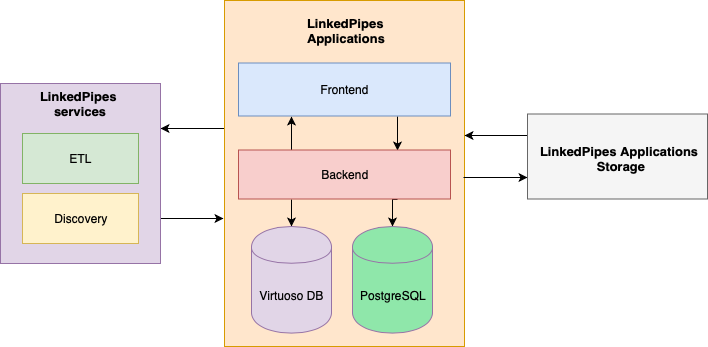
\includegraphics[width=14cm]{lpa_highlevel_architecture.png}
    \caption{High-level overview of LinkedPipes Applications Platform}
    \label{fig:lpa-high-level-arch}
\end{figure}

Generally, we can categorize it into three main parts: 

\begin{itemize}
    \item \textbf{\lpa{}} - the main platform from LinkedPipes bundle, and the main stakeholder for \lpas{} project. Combines multiple database solutions for LinkedData, conventional SQL for storing user related records and implementation of a backend and frontend for creating applications.
    \item \textbf{LinkedPipes Services} - a set of external services provided from LinkedPipes bundle that \lpa{} heavily utilizes. Provides a toolset for identifying how linked data can be discovered, extracted, transformed and loaded into an RDF file for further processing.
    \item \textbf{\lpas{}} - the main goal of the following thesis and a functional storage solution for \lpa{} platform. Contains a set of API controllers and managers that allow users of \lpa{} to store and share their applications in a secure and decentralized way. Consecutive chapters will provide a detailed overview of an architecture and implementational details.
\end{itemize}

\subsection{\lpa{}}

\subsubsection{Frontend}

\subsubsection{Backend}

\subsubsection{Virtuoso DB}

\subsubsection{PostgreSQL} 

\subsection{LinkedPipes Services} 

\subsubsection{Discovery} 

\subsubsection{ETL} 

\subsection{\lpas{}}

\section{Functional requirements}

The following sections describes the main functional requirements defined for the \lpa{}. 

\subsection{User authentication}

The user of the platform should be able to register an account in the application, log in and log out. Moreover, once logged in, the platform should be provide functionality to create, configure and publish applications visualizing LinkedData. However, to view an application, it is not necessary to be logged in or even registered.

\subsection{Create Application}

The Create Application functionality could be described as a core feature of the LinkedPipes Application.

The platform needs to provide the a tooling to specify the data sources to be utilized so that an instance of an interactive application would be created based on provided data sources. In addition to that, there needs to be four ways to provide the data source:

\begin{itemize}
\item Provide a set of dataset \acrshort{IRI}s which the tool will de-reference to get the dataset.
\item Specify a \acrshort{SPARQL} endpoint from which data will be queried and extracted.
\item Upload a file in \acrshort{TTL} format, containing data source specifications.
\item Use some sample dataset provided by the tool
\end{itemize}

\subsection{Configure Application}

After the creation of the application, platform also need to provide functionality to configure previously created applications. Each application, depending on the visualization, will have particular settings that can be set. Furthermore, users must be able to control, with the use of filters, which data is to be used and displayed. The available filters should be automatically derived based on the properties and semantics of the data. 

The set of configure operations for filters can be described as follows:

\begin{itemize}
\item Removing whole data filters to ignore the values of specific data properties.
\item Removing selected values of some filters.
\item Setting fixed values for some filters.
\item Set/change a name for the application.
\end{itemize}

\subsection{Publish Application}

Another important requirement is an ability to publish the application and make it publically available for sharing the visualization to anyone via the permanent link. Furthermore, when a third party accesses this \textit{permalink}, the browser should open the LinkedPipes Applications website with the respective application opened, as configured by the publisher.

Besides, when publishing an application I want the tool to offer the possibility to choose one of the below two settings:

\begin{itemize}
\item Use and display cached data, making the published application a fixed view.
\item Regularly refresh the data from the previously chosen data sources of the interactive application.
\end{itemize}

The tool will also need to provide the ability to embed the published view into a data journalist's web page, for example, using an iFrame.

\subsection{Store Application}

Since published applications require to be publically accessible to anyone, the platform needs to have a functionality to persist the configurations of the applications in a secure way. Moreover, the configurations for most of the published applications are represented as LinkedData, therefore the persistent storage tooling needs to be optimized for files in RDF format. 
User needs to be able to browse the stored and published applications and optionally allow other people to collaborate or edit a specific shared application. 

% A detailed overview of the solution as well as the overview of current alternatives to \solid is provided in the consecutive chapters of this thesis. 
\chapter{Related work}
\label{chap:num_2}

This chapter provides an overview of currently available alternatives to \solid{} project, as well as research projects that share similarities with the core concepts of decentralized social platforms. The first set of sections provides a general description of alternative technologies, the last \autoref{sssec:comparison_of_technologies} provides a comparison between the alternative software solutions and \solid{}.

\section{Diaspora}

Out of all currently available solutions, the conceptually closest software platform to \solid{} is Diaspora \cite{diaspora_paper}\cite{diaspora_site}. In general, it is a decentralized social network platform that enables users to choose the server where their data is hosted and even run their own data hosting server. In that sense, it is similar to \solid{}. However, the main focus in Diaspora is to act as a social network, where social data is shared between users using specific APIs, and not running diverse applications on stored data. Unfortunately, it does not offer a well-defined way to use the same data with different applications. Note that Diaspora uses the term pod to refer to a data hosting server. A Diaspora POD is what \solid{} would refer to as a \solid{} server.

\section{WebBox}

WebBox is a decentralized social network platform that decouples data from applications \cite{webbox}. As \solid{}, it stores user’s data as Linked Data in a decentralized way. Also similar to \solid{}, system rely on WebID for decentralized identity, authentication, and access control. In WebBox, each data storage service exposes a SPARQL endpoint, and applications manipulate the data via SPARQL queries and updates, or via HTTP GET requests. In contrast, \solid{} offers the full power of LDP for simple data interactions (e.g., hierarchical data organization, fine-grained manipulation) and additionally allows the use of link-following SPARQL for complex data retrieval. It also works as a generic storage platform upon which a significantly larger number of applications can be built. As a last remark, WebBox was mainly mentioned due to the similarities in functionality with \solid{} project, however, the platform was never released out of the bounds of a research prototype.

\section{OwnCloud}

OwnCloud \footnote{\url{https://owncloud.org}} is a self-hosted open source file sync and share server. In regards to previously defined requirements, this solution is somewhat too generic to the goals of the project, but due to certain features such as decentralization of the storage using manually setup instances, and various scalability features, building a platform based on the provided API is possible. Similar to Dropbox, Google Drive, Box, and others, ownCloud lets you access your files, calendar, contacts, and other data. You can synchronize everything between your devices and share files with others. In contrast with \solid{}, the solution is still a generic cloud storage. It does not support Linked Data out of the box and does not provide a trivial way to decouple data from applications using the data. 

\section{Mastodon}

Mastodon is an online, self-hosted social media, and social networking service \cite{mastodon}. It allows anyone to host their own server node in the network, and its various separately operated user bases are federated across many different sites (called "instances"). These instances are connected as a federated social network, allowing users from different instances to interact with each other seamlessly. Mastodon is a part of the wider Fediverse, allowing its users to also interact with users on other platforms that support the same protocol, such as PeerTube, Misskey, Friendica and Pleroma.

Mastodon has microblogging features similar to Twitter, or Weibo, although it is distinct from them, and unlike a typical software as a service platform, it is not centrally hosted. Each user is a member of a specific, independently operated instance. Users post short messages called "toots" for others to see, and can adjust each of their post's privacy settings. The specific privacy options may vary between sites, but typically include direct messaging, followers only, public but not listed in the public feed, and public and posted to the public feed. The Mastodon mascot is a brown or grey woolly mammoth, sometimes depicted using a tablet or smartphone.

Because there is no central server for Mastodon, each instance has its own code of conduct, terms of service, and moderation policies. This differs from traditional social networks by allowing users to choose an instance which has policies they agree with, or to leave an instance that has policies they disagree with, without losing access to Mastodon's social network.

\section{Hubzilla}

Hubzilla \footnote{\url{https://fediverse.party/en/hubzilla/}} is a modular webserver based operating system which includes technologies for publishing, social media, file sharing, photo sharing, chat and more (including the ability to develop custom modules). These services are accessed and connected across server and administrative boundaries through the communication protocol Zot which provides a high level of privacy and security customization and a nomadic identity for the users. A webserver running Hubzilla is called a "hub".

\section{Centralized cloud storage solutions}

Modern commercial and enterprise cloud storage solutions provide a great set of features as platforms for any generic use cases when reliable file storage is needed. For instance, Google Cloud Storage \footnote{\url{https://cloud.google.com/storage/}} and Amazon AWS Storage \footnote{\url{https://aws.amazon.com/products/storage/}}. However, in contrast with \solid{}, this approach is the most distant from the main concepts of LinkedPipes Applications project’s requirements. As a main disadvantage of the approach is the fact that even though the developer is offered a great set of flexibility within the platform, the data storing aspects are not fully decentralized. It also means that the end-user is uploading his data into a centralized data silo where commercial terms of services policies regulate ownership of his data. Another issue is platform dependency meaning that migrating, sharing, and interchanging the data between platforms is not trivial since all interactions with data within storage are defined by a set of APIs and SDKs specific to the selected platform. 

\subsection{Pitfals of centralized cloud storages}

In the past, having control over content or information people store and access online was a common case for many technologies on the Web. However, during the past 20 years, that situation changed significantly. Various tech giants and media platforms like Facebook and Google gain control over the personal data of millions of users using their services. The data that is under the control of the fixed authority separated from the rest of the organization or community is often referred to as data silos.  From the standpoint of the company, having centralized control over the data of all users of their platforms brings many benefits. It simplifies the development of services within the organization, allows to perform various analytics processes and understand the users better. However, from the users perspective, it significantly reduces the control of their data stored within centralized platforms.

\section{Comparison of technologies}
\label{sssec:comparison_of_technologies}

A significant difference between Solid and services mentioned below is that \solid{} sets a standard way of operating through a data model (RDF) and does not dictate how instances should behave as part of a "federation". In addition to that, \solid{} is not just a software technology, and it represents specifications built on top of open web standards, an extensive set of guidelines for developers, a community of active researchers and contributors. When it comes to direct comparison, \solid{} could be defined as a lower-level abstraction than federated services like Diaspora and Mastodon in the sense that \solid{} can serve as an infrastructure for building those platforms. For instance, Diaspora and Mastodon could be integrated into Solid by allowing their users to sign in using their WebID, and then allow users to store the data produced by them on the services on their POD. 

\begin{table}[hbt]
\centering
\resizebox{\textwidth}{!}{%
\begin{tabular}{|c|c|c|c|c|c|c|}
\hline
\textbf{Technology} & \textbf{\begin{tabular}[c]{@{}c@{}}Provides Personal \\ Data Store?\end{tabular}} & \textbf{\begin{tabular}[c]{@{}c@{}}Is stored data\\ easily reusable?\end{tabular}} & \textbf{\begin{tabular}[c]{@{}c@{}}Has decentralized\\  infrastructure?\end{tabular}} & \textbf{\begin{tabular}[c]{@{}c@{}}Has Linked Data \\ support?\end{tabular}} & \textbf{\begin{tabular}[c]{@{}c@{}}Is Open \\ Source?\end{tabular}} & \textbf{\begin{tabular}[c]{@{}c@{}}Is used in \\ production?\end{tabular}} \\ \hline
\solid{} & Yes & Yes & Yes & Yes & Yes & No \\ \hline
Diaspora & Yes & No & Yes & Yes & Yes & Yes \\ \hline
WebBox & Yes & Yes & Yes & Yes & No & No \\ \hline
OwnCloud & No & No & No & No & Yes & Yes \\ \hline
Mastodon & No & Yes & Yes & No & Yes & Yes \\ \hline
HubZilla & Yes & Yes & Yes & No & Yes & Yes \\ \hline
\begin{tabular}[c]{@{}c@{}}Popular centralized cloud \\ storages\end{tabular} & No & No & No & No & No & Yes \\ \hline
\end{tabular}%
}
\label{tab:solid_comparisons_table}
\caption {A comparison table between \solid{} and alternative technologies with similar concepts.}
\end{table}

% TOD : hot to fix the table autoref ?

The table \TODO{use autoref} \ref{tab:solid_comparisons_table} provide a detailed comparison between \solid{} and technologies alternative to it. The columns indicate questions representing main features required from a technology to be able to use the benefits of Semantic Web, Linked Data, and RDF at full scale while preserving security and decentralized storing aspects. Both Diaspora and WebBox come very close to \solid{} in terms of provided functionality. However, as mentioned in their descriptions, Diaspora does not focus actively on storage and data decoupling aspects, and WebBox is a proof of concept project that is not available in production or has an open-source community. Similar to Diaspora, Mastodon and Hubzilla position themselves as platforms providing various social networking features to users. And finally, solutions like OwnCloud or popular centralized cloud storage solutions from Google, Microsoft, or Amazon provide convenient developer APIs for using their technologies. However, the technology itself does not preserve the ideas of decentralization and privacy-oriented data management. In contrast, as mentioned before, it provides an opposite functionality where data gets aggregated inside centralized silos under control of the organization providing the storage. 
To sum up, this section provided a brief comparison overview of alternatives to \solid{}. The following \autoref{chap:num_3} will give detailed reasoning for choosing \solid{} as a core technology for providing storage capabilities for \lpa{} and what makes it a better fit than its alternatives. 

\chapter{Analysis}
\label{chap:num_3}

The following chapter will start by providing a detailed set of functional and non-functional requirements from \lpa{} in regards to \lpas{}. Afterward, an analysis of the currently available development tools within the \solid{} ecosystem will be demonstrated. Additionally, as a continuation of comparison in \autoref{sssec:comparison_of_technologies}, a reasoning for choosing \solid{} as a core technology for implementing \lpa{} requirements will be explained.  The majority of the functionality of \lpa{} and \lpas{} were implemented by the author while working in parallel as a part of \lpa{} and as an individual contribution to the thesis. Therefore, to simplify the understanding of work on both projects and the difference between both contributions, the whole chapter is structured under the assumption that \lpa{} is a stakeholder with a working solution and \lpas{} is a technology yet to be implemented and integrated into \lpa{}. The consecutive chapter on architecture in \autoref{chap:num_4} and the implementation in \autoref{chap:num_5}, will guide the reader through established software development cycles where the result will be provided as a summary of implementation details in regards to requirements defined in this chapter.

Aside from definitions of specific requirements, it is important to note that there are three main \textit{actors} involved in statements of requirements. An actor is an individual entity interacting with the software components in requirements. Specific types are defined as follows:
\begin{itemize}
    \item \textit{Data journalists}, this category of actors are one of main target users of \lpa{} platform. They are defined as people familiar with, at least, basics of Semantic Web. They can provide Linked  Data sources to \lpa{} for further visualization and publishing of apps. They are also assumed to have an actual account in the \lpa{} platform.
    \item \textit{Lay users}, this is a second target category of users of \lpa{} platform. They do not have any prior experience with Semantic Web and in most cases, browse the published visualizers created by Data journalists. They are not obliged to have an actual account in the \lpa{} platform.
    \item \textit{\acrfull{LPA} Developers}, a developers implementing on \lpa{} platform codebase and main users of \lpas{} features, APIs and functionality to be developed. The majority of details in \autoref{chap:num_5} are focused on developing a developer-friendly software for this category of users.
\end{itemize}

\section{Functional requirements}
\label{ssec:functional_requirements}

In general, every functional requirement is defined as a description of services or features that software must offer. In this case \lpa{} defines a set of features expected to be handled properly by the \lpas{} project. The requirements are provided as a set of UML use-case \footnote{\url{https://www.uml-diagrams.org/use-case-diagrams.html}} diagrams as well as formal textual descriptions. 

\subsection{User authentication}

The user of the platform should be able to register an account in the application, log in, and log out. The requirement might seem unfitting to the purposes of \lpas{}. However, if \solid{} is considered to be used, it provides the fully functional authentication mechanisms based on WebID that can be used for generic platform authorization.

\begin{figure}[h]
\centering
\fcolorbox{black}{white}{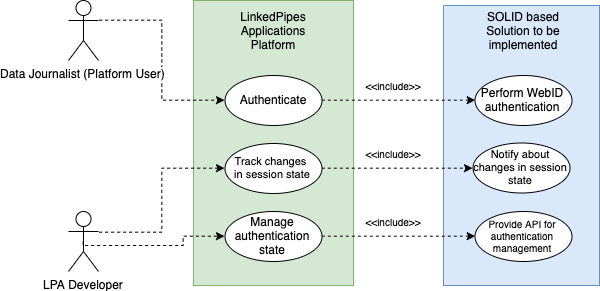
\includegraphics[width=0.7\linewidth]{lpa_authenticating_use_case.png}}
\caption{A UML use-case diagram describing user authentication requirement.}
\label{fig:lpa_authenticating_use_case}
\end{figure}

The UML diagram on \autoref{fig:lpa_authenticating_use_case} is described as follows:
\begin{itemize}
    \item \textit{Authenticate}, a platform must provide a way for Data Journalists (Platform Users) to authenticate via \lpa{} platform. This assumes that \lpa{} platform has an ability to communicate with the storage solution either integrated into \lpa{} codebase or presented as entirely separate service and \textit{perform WebID authentication}.
    \item \textit{Track changes in session state}, a platform must provide an API or a developer library for tracking any changes in the state of the authenticated platform user session. This assumes that the storage solution can inform the \lpa{} platform about such changes.
    \item \textit{Manage authentication state}, the platform must provide an API or a developer library for managing the authentication state of the users. This assumes that the core functionality is provided by the storage solution that exposes an API or a developer library toolset for developers to perform such interactions.
\end{itemize}

\subsection{Create, Store and Publish Application}

Creation, storing, and publishing of the application are the core features provided by the \lpa{} itself. However, the storage aspects are involved a lot when it comes to storing the created app. Consequently, publishing also consists of interacting with storage since an end-user expects the storage solution to have an identifier for his stored application.

\subsubsection{Creating and storing application}

User should be able to create an application within the \lpa{} platform and store it in his personal space in an authenticated storage. The storage solution can either implement a solution that stores entire application including the visualizer or generates a metadata configuration file that allows to re-create the entire application within \lpa{} platform from scratch.

\subsubsection{Publishing an application}

Another important requirement is an ability to publish the application and make it publically available for sharing the visualization to anyone via the permanent link. Furthermore, when a third party accesses this \textit{permalink}, the browser should open the \lpa{} website with the respective application opened, as configured by the publisher. The tool will also need to provide the ability to embed the published view into a data journalist's web page, for example, using an HTML \texttt{iframe} \footnote{\url{https://html.com/tags/iframe}}. 

\subsubsection{A diagram overview}

The \autoref{chap:num_5} describes the specific of creation, storing and publishing application requirements from perspectives of different actors involved. 

\begin{figure}[h]
\centering
\fcolorbox{black}{white}{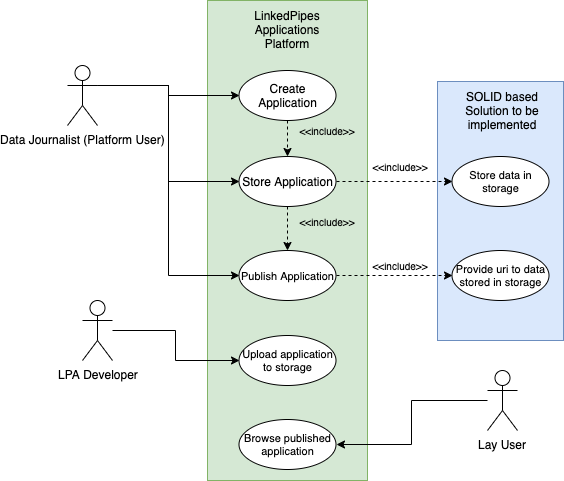
\includegraphics[width=0.6\linewidth]{lpa_creating_apps_use_case.png}}
\caption{A UML use-case diagram describing creation, storing and publishing application requirements.}
\label{fig:lpa_creating_apps_use_case}
\end{figure}

The diagram is described as follows:
\begin{itemize}
    \item \textit{Create application}, the platform provides an ability for Data Journalists to create an application. The process of creation of an application within \lpa{} also assumes that it is consequently \textit{Stored} and \textit{Published} via a set of interactions with storage. The publishing process is extended from storing an application because to publish an application, a configuration needs to be saved, and a URI for a stored resource in a \solid{} POD is extracted.
    \item \textit{Upload application to storage}, a platform provides an API or a library for LPA Developers to perform uploading of an application into the storage solution.
    \item \textit{Browse published application}, a platform provides a way for any Lay User to browse the published application created by Data Journalists. This is included as a part of the requirement since publishing is directly interacting with storage, and implementation of the requirement applies to both \lpas{} and \lpa{} platform.
\end{itemize}


\subsection{Managing storage and sharing published applications}

The last set of requirements is related to storage management and the sharing of published applications. The storage management requires a functionality that allows platform users to \textit{move}, \textit{copy} and \textit{create} data in their authenticated spaces in storage. The sharing requirement describes the functionality to allow users to share the applications they have published and control the access control settings to them. Since published applications require to be publically accessible to anyone, the platform needs to have a functionality to persist the configurations of the applications in a secure way. Moreover, the configurations for most of the published applications are represented as Linked Data. Therefore the persistent storage tooling needs to be optimized for files in RDF format.
 
\begin{figure}[h]
\centering
\fcolorbox{black}{white}{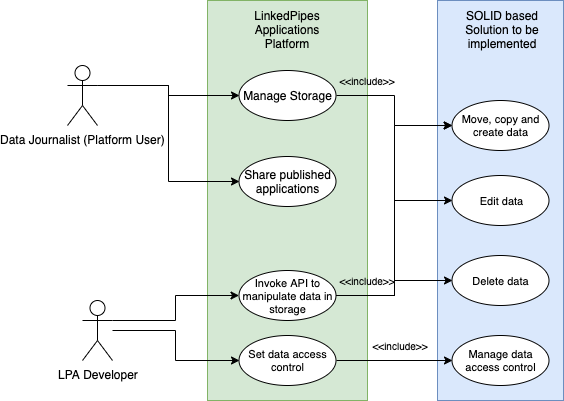
\includegraphics[width=0.6\linewidth]{lpa_managing_storage.png}}
\caption{A UML use-case diagram describing requirements on storage management and sharing of published application.}
\label{fig:lpa_managing_storage}
\end{figure}

As demonstrated on \autoref{fig:lpa_managing_storage}, the main elements are described as follows:
\begin{itemize}
    \item \textit{Manage storage}, the functionality of the platform to allow Data Journalists (Platform Users) to interact and manipulate data in their storage. In the case of \lpa{}, it is limited to visualizer application-related data only. 
    \item \textit{Share published applications}, an ability for Data Journalists to share the application with other users of the \lpa{} platform and set access control to the published applications.
    \item \textit{Invoke API to manipulate data in storage} assumes that \lpa{} provides tooling for their developers to interact with storage solution and invoke its APIs or libraries for manipulating data.
    \item \textit{Set data access control}, assumes that \lpa{} provides tooling for their developers to interact with storage solution and invoke its APIs or libraries for editing access control privileges to data.
\end{itemize}

\section{Non-functional requirements}
\label{ssec:non_functional_requirements}

In general, every non-functional requirement is described as the quality attributes of a software system, which contrasts with functional requirements that are specific to the exact behavior of the system. Within the scope of \lpa{} platform, the stated non-functional are rather an informal set of terms mainly related to \textit{reusability}, \textit{testability} quality attributes. 

\subsection{Compatibility with latest tools}

This general non-functional requirement states that an implemented software solution should be compatible with the latest tools of its technological ecosystem. For instance, if the designed software is a library using third-party packages, it needs to be generic enough to be compatible or have mechanisms to be resilient to any significant changes in third-party packages that it relies on.

\subsection{Clean APIs and libraries}

The solution needs to be implemented with code readability and reusability in mind. The primary users of the solution are developers of \lpa{} platform. Therefore it is essential to have an implementation based on a design that minds the established best practices and patterns of software engineering. 

\subsection{Continuous Integration and Delivery}

The implemented solution needs to maintain an optimized and fully automated Continuous Integration and Delivery pipelines. This ensures better possibilities in gaining contributors and planning future work and improvements on the solution as well as an infrastructure to debug and fix errors more effectively.

\subsection{Easy integration with \lpa{}}

The final solution needs to be able to integrate with the \lpa{} easily. Another important aspect is the solution to be integrated should not be entirely tied to the specified \lpa{} platform and should have the potential to be reused in other Linked Data based applications.

\subsection{Decentralized storage}

The Data Journalists, one of the primary target users of \lpa{} platform, should be able to choose any storage that is compliant with the technology stack of the solution. In other words, the platform should be able to support storing data in any personal space of such storage instances that are created, hosted, or owned by users directly or by the third-party providers.

\section{\solid{} development toolset}

Now, as the main requirements of the \lpa{} platform are defined, let us dive into the analysis of the \solid{} technology and tooling that it provides to understand better how it can be used to cover all stated requirements.

At the core \solid{} is a set of open specifications. At the current state of the project implementation, the community is most concerned about the persistence and representation of resources. However, such aspects as identity, authentication, and authorization are also vital parts of \solid{}.

A set of these standards are undergoing active implementation stage. Main contributors consisting of the core \solid{} development team, as well as the open-source community, develop the standards into various servers and tools. For instance, a \texttt{node-solid-server} library that implements a Solid server in Node and \texttt{rdflib.js} that allows you to manipulate RDF programmatically.

In addition to this, there is work done on supporting tools, such as Solid React SDK, that is created to allow developers to more easily get into developing apps with Solid. As part of this is the style guide that can be reused by others, not wanting to use the React parts.

\subsection{The \solid{} servers}

\solid{} itself represents a tech stack of complementary standards and data format vocabularies that are currently only available in centralized social media services. It also represents a Specification Document, serving as the main guideline for developers building their own apps and services. However, aside from that \solid{} also refers to a set of servers that implement its specification. 

\subsubsection{gold}

\texttt{gold} is a reference Linked Data Platform server for the \solid{} platform. The implementation is written in Go, based on initial work done by William Waites \cite{solid_gold_server}.

\subsubsection{node-solid-server}

Following solution is an implementation of a server based on \solid{} specifications in Node.js \cite{node_solid_server}.
One of the main advantages is that it could be launched as a \solid{} server on top of the local file-system. Interaction with server can be performed as follows:
\begin{itemize}
	\item Command line tool.
    \item Via \texttt{node-solid-server} library.
\end{itemize}

The provided server implementation was used as a main \solid{} server for the project due to compliance with main requirements for choosing the server. Those can be described as follows:
\begin{itemize}
	\item \textbf{Easy integration with current \lpa{} project}, specifically the frontend web project. This allows usage of provided `node-solid-server.js` library.
    \item \textbf{Active maintenance by open-source community}. Aside from that, this server implementation is considered to be a default option suggested by creators of \solid{}.
    \item \textbf{Support of \textit{WebID-TLS} and \textit{WebID-OIDC}}. This implies majority of WebID communications protocols,
    crucial to the user authentication and security aspects of the storage within \lpa{}. The WebID-TLS stands for a WebID authentication method over \acrfull{TLS}, providing an efficient and user friendly authentication on the Web \cite{webid_tls}. The WebID-OIDC is an authentication delegation protocol suitable for WebID-based decentralized systems such as \solid{} \cite{webid_oidc}.
\end{itemize}

\subsection{The \solid{} React development stack}

The main frontend library used in LinkedPipes Applications is React. In order to incorporate easier integration of aspects of \solid{} into the project, an analysis of React related \solid{} frameworks and libraries was performed. Even though, \solid{} community is yet to grow become stable and mature, it already provides a convenient set of libraries for React that were used as a main tools during implementation of the thesis project. 

\subsubsection{solid/react}

The main purpose of this library is to provide the following functionality:

\begin{itemize}
	\item Provide React developers with components to develop \solid{} apps.
    \item Enable React developers to build their own components for \solid{}.
\end{itemize}

\subsubsection{@inrupt/solid-react-components}

This libray is an official SDK provided by Inrupt for developing React Web applications for \solid{}. The package include various dependencies allowing:

\begin{itemize}
	\item Provide React developers with a set of easily customizable components interacting with \solid{} specifications.
    \item Provide a standardized visual design conventions based on Atomic Style.
    \item A set of cli commands for generating a template \solid{} projects.
\end{itemize}

\subsubsection{solid-auth-client}

The main purpose of this low level library is to provide ability to easily perform Authentication operations while interacting with \solid{} pods and servers.

At its core it is a browser library that allows your apps to securely log in to \solid{} data pods and read and write data from them.

\subsubsection{solid-file-client}

This library provides a simple interface for logging in and out of a Solid data store, maintaining a persistent session, and for managing files and folders. It may be used either directly in the browser or with node/require. The library is based on solid-auth-client and solid-cli, providing an error-handling interface and some convenience shortcuts on top of their methods and providing a common interface to the two modules.

\subsubsection{rdflib}

JavaScript RDF library for browsers and Node.js. One of the main contributors is Sir Tim Berners-Lee himself. The library is going to be used and described in detail in \autoref{chap:num_5}.

\subsubsection{@solid/query-ldflex}

The following library adds support of the LDflex language to \solid{} by:

\begin{itemize}
	\item Providing a JSON-LD context for \solid{}.
    \item Binding a query engine (Comunica).
    \item Exposing useful data paths.
    \item LDflex expressions occur for example on Solid React components, where they make it easy for developers to specify what data they want to show. They can also be used as an expression language in any other Solid project or framework.
\end{itemize}

\section{Why \solid{}?}
\label{sssec:why_solid}

Even though it is presented as a flawless dominating technology in \autoref{table:solid_comparisons_table}, it is, in fact, far from being perfect. Some of the disadvantages include:
\begin{itemize}
    \item \textit{Still under active research and development}, the project itself started back in 2016. Still, the real active traction and improvements had happened only within the past two years after community grew bigger, and the project gained popularity in the open-source community. It also means that there are still major changes in specifications introduces in every new iteration.
    \item \textit{Lack of actively maintained community libraries}, even though \solid{} organization on GitHub \footnote{\url{https://github.com}} actively updates and maintains its libraries for interacting with \solid{}. There is a large number of libraries developed by the community with tools that, in some cases, are more useful and popular. However, due to the \solid{} project still being actively developed, a lot of libraries outside of the scope of the organization become obsolete and outdated quickly.
    \item \textit{Still a lot of room for improving infrastructure for developers}. The project does not provide intuitive and user-friendly documentation. An average developer is required to have basic knowledge in Semantic Web, Linked Data, and working with RDF and SPARQL. However, the improvements were made in 2019, and eventually, the onboarding process into the technology will become easier for any developer.
\end{itemize}

Despite the disadvantaged mentioned above, the main reason for choosing \solid{} as a core for providing storage capabilities to \lpa{} was the fact that it is a very flexible and low-level technology.  Firstly,  as mentioned earlier, \solid{} represents multiple things at once. It is both a toolset with libraries for developers, a set of specifications, and an ambitious idea to a better World Wide Web where people own their data, and all information is linked together, preserving the semantic meaning. Of course, many attempts on decentralization were made before, but \solid{} differs from the others in the way that it does not target individuals in specific fields or domains of the Internet, it attempts to change the Internet itself, making it a better online space for everyone. And lastly, it demonstrated itself as a perfect fit for any application that requires any social aspects and involves dealing with any form of Linked Data, where \lpa{} platform and its requirements are compliant to all of the statements mentioned earlier.
\chapter{Architecture}
\label{chap:num_4}

The following chapter provides an overview of the architecture of \lpas. Explains the main components of the Storage as well as how it is being integrated into the LinkedPipes Applications platform.

\section{High-Level Overview}

While the majority of components were described in detail in \autoref{chap:num_1}, the overview architecture provided in this section shows more specific details on how all the external and internal components of the system are interacting. One of the essential details represented in the figure \ref{fig:lpas_high_level_architecture} is the separation between codebases of \lpa{} and \lpas{}. The \lpa{} Frontend imports the \lpas{} as an npm \footnote{https://www.npmjs.com} package and performs all interactions with \solid{} using the provided functionality of the package. In some sense, \lpas{} is being treated as an additional rudimentary backend and database layer on top of existing internal components inside \lpa{}. This is due to several functional requirements that \lpas{} package implements, such as \textit{user authentication}, \textit{operations to manipulate resources inside storage} and etc.

\begin{figure}[h]
\centering
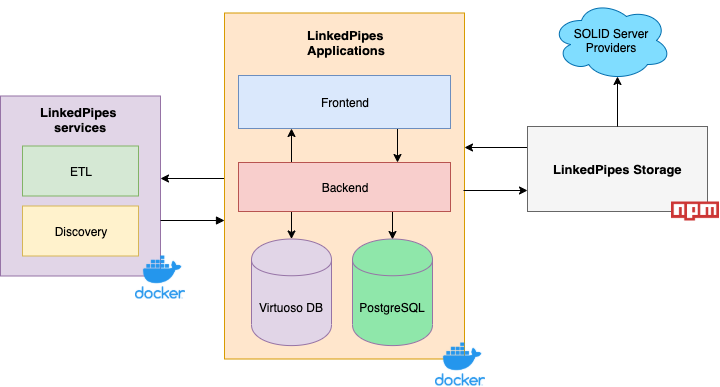
\includegraphics[width=14cm]{lpas_high_level_architecture.png}
\caption{High level overview of \lpa{} and \lpas{} interactions}
\label{fig:lpas_high_level_architecture}
\end{figure}

As additionally demonstrated, the figure \ref{fig:lpas_high_level_architecture} also has Docker icons displayed under some modules. The icons indicate where the production-ready service is hosted. For instance, in the case of the \lpas{}, the end goal is the npm registry, while \lps{} and \lpa{} are all hosted in the docker registry where each internal component is a docker container.
The generic interaction flow usually involves direct communication between the \lpa{} frontend and \lpas{} package. The internal frontend component has various React components implemented using the \lpas{} package that provides navigation and interaction with \solid{} Pods. While the package is designed under the assumption that the \lpa{} is the only user of the package, some abstractions are generic enough and have the potential to be used outside of the scope of the main functional requirements. The implementation chapter will also cover a generic use-case on how quick start \CONSIDER{how to start quickly} with application development based on \solid{}.

\subsubsection{The evolution of solid specifications}
At the moment of writing this chapter, the official \solid{} specification reached version \texttt{0.7.0} \footnote{\url{https://github.com/solid/solid-spec/blob/master/CHANGELOG.md}}. Introducing many changes and improvements, it also adds an extra layer of complexity with every release, changing some of the conventions, or updating some fundamental paradigms. As a result, when \lpa{} was initially implemented, it was based on an older specification and older versions of \texttt{node-solid-server}, that had a simpler and more extensive ability to manipulate ACL files. The work within this project, however, was focused around putting efforts into making it generic enough so that people could use it as a guideline for any started \solid{} apps, while the implementation will fit all \lpa{} requirements.

The main note to mention for the further section in this chapter is that the architecture design was derived from relying on the official specification of \solid{} while also referring to the provided functionality of \texttt{NSS} that does not always strictly follow the guidelines in the specification. 


\section{Storage}
\label{ssec:storage}

The initial architecture and implementation draft of \lpas{} were different from what is presented in this chapter.  \solid{} related logic was firstly a part of the \lpa{} codebase. Therefore, significantly complicating unit testing and making it hard to define the scopes of the \lpa{} and \lpas{} projects implementation. Later on, a decision was made to separate the logic of the \lpas{} and move it in the separate codebase. The majority of abstractions that were initially designed to be inside the \lpa{} codebase, consisted of various wrappers and crud functions to interact with \solid{} servers. Their design was refined and aggregated into specific abstractions, each responsible for covering the functional requirements from \lpa{} project.

\begin{figure}[h]
\centering
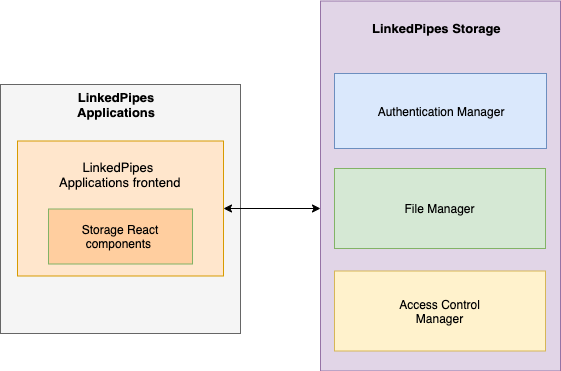
\includegraphics[width=14cm]{lpas_high_level_abstractions.png}
\caption{Main abstractions of \lpas.}
\label{fig:lpas_high_level_abstractions}
\end{figure}

Let us start by describing the main abstractions providing the functionality of \lpas{}.

\subsection{Authentication Manager}
\label{sssec:authentication_manager}

The Authentication Manager is responsible for wrapping \solid{} WebID based authentication logic into a simple and developer-friendly abstraction At the moment of writing this, the official \solid{} specification states to support the following protocols:
\begin{itemize}
\item WebID-TLS  - is one of the primary authentication protocols that rely on WebIDs instead of usernames. The passwords are replaced with certain cryptographic certificates as bearer tokens and are stored within the user's browser.
\item WebID-OIDC - alternative authentication protocol based on OAuth2 and OpenID Connect protocols and adjusted to support the concept of WebID. This is, in fact, the first authentication option provided by \lpas{}, later chapters will provide the reasoning behind why this ended up being a more intuitive option to cover the authentication requirement for \lpa{}.   
\end{itemize}

As already mentioned in chapter \ref{chap:num_3}, the usage of \textit{WebID} protocols is one of many benefits of \solid{}, in contrast with popular authentication protocols used in centralized silos, it is completely agnostic to specific authentication mechanisms, allowing our single abstraction to support any arbitrary \textit{WebID-OIDC} compliant \solid{} provider. 


\subsubsection{Interacting with frontend}

Sequence diagram on \autoref{fig:lps_authentication_sequence_diagram} demonstrate an example on how the Authentication Manager will be used within the \lpa{} Frontend and how it will interact with \solid{} Providers. The user agent entity represents a typical lay \lpa{} user interacting with the platform through the frontend component. The sequence flow consists of the following steps:

\begin{enumerate}
    \item The user clicks on the 'Authenticate' button. This is the starting point of this sequence diagram that serves as a trigger for \lpa{} to invoke the \lpa{} package.
    \item The frontend component calls the Authentication Manager and awaits for a callback. As the main input, it supplies the information about the \solid{} provider that the user would like to use.
    \item The Authentication Manager contacts the \solid{} provider and requests the provider authentication web page. Each provider conforming to \solid{} specification should contain that page.
    \item Depending on the browser environment of the user, he gets redirected to the provider's authentication web page either in a new browser tab or a popup dialog.
    \item The user selects the preferred authentication and inputs the credentials. At the moment of writing this thesis, popular \solid{} server implementations like node-solid-server support both WebID+TLS and WebID-OIDC specifications.
    \item The Authentication Manager receives the callback from the provider and sets the authenticated user session token.
    \item Frontend component receives the callback from the Authentication Manager, indicating that the user is authenticated.
    \item As the last step, the frontend redirects the user into the homepage dashboard of \lpa{} platform.
\end{enumerate}


\begin{figure}[ht]
\centering
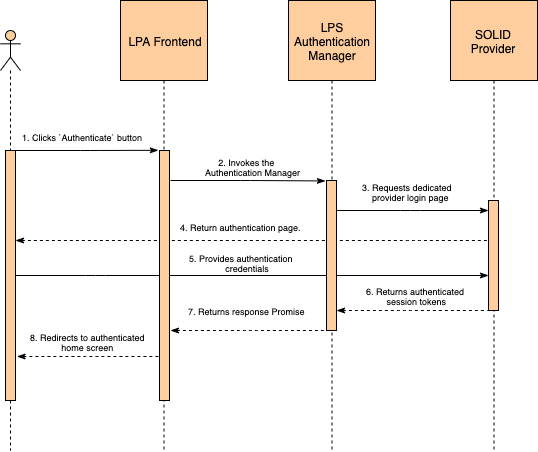
\includegraphics[width=12cm]{lps_authentication_sequence_diagram.png}
\caption{Sequence diagram for \textit{authenticate} operation invoked from \lpa{} frontend.}
\label{fig:lps_authentication_sequence_diagram}
\end{figure}


\subsection{File Manager}
\label{sssec:file_manager}

The File Manager is responsible for implementing the CRUD operations for the \solid{}  providers that are compliant with Linked Data Platform specification. The \gls{LDP} is a specification that is reused and extended in the \solid{} specification to describe the REST API for interacting with LDP Resources and LDP Containers \cite{lpd_specification}. LDP Resources and LDP Containers are, in some sense, the basic building blocks of any \solid{} POD, since they allow users to create any files and folders. 

As mentioned earlier, the \solid{} specification is re-using the LDP specification to provide a RESTful set of operations to interact with any compliant implementation of that specification. 

The LDP has an extensive set of resource types that are suited for defining the folder and files. However, the architecture provided is relying on two common resource terminologies that were simple enough to cover the requirements without complicating the design of the architecture. Those resources are defined as follows:

\begin{itemize}
%    Cite resource 
     \item Linked Data Platform Basic Container (LDP-BC), is a Linked Data Platform Basic Container. An LDP-RS representing a collection of linked documents that respond to client requests for creation, modification, and enumeration of its linked members and documents, and that conforms to the simple lifecycle patterns and conventions.
    \item An HTTP resource whose state is represented in any way that conforms to the simple lifecycle patterns and conventions, in other words any resource that can be \textit{created}, \textit{updated}, \textit{deleted} and \textit{red}. The LDP servers process the CRUD operations to manipulate the lifecycle of LDPRs.
\end{itemize}


\subsubsection{Creating resources}

The essential operation that is at the core of most functional requirements defined earlier is the ability to create a resource in a POD. Using the NSS server as a basis, the general convention for creating LDP resources is a POST HTTP request providing a link to the POD using the path where resource needs to be created. As demonstrated on \autoref{fig:lpas_create_resource} the creation consist of the following steps:
\begin{enumerate}
    \item \lpa{} frontend invokes the FileManager abstraction with a request specified in \texttt{ResourceConfig} abstraction. The configuration provided contains information on the type of resource, whether it is a folder or a file. Additionally, it describes the required information to identify the resource within the POD.
    \item \lpas{} constructs an HTTP POST request to create the resource in POD in \solid{} server, the response is forwarded asynchronously.
\end{enumerate}

\begin{figure}[h]
\centering
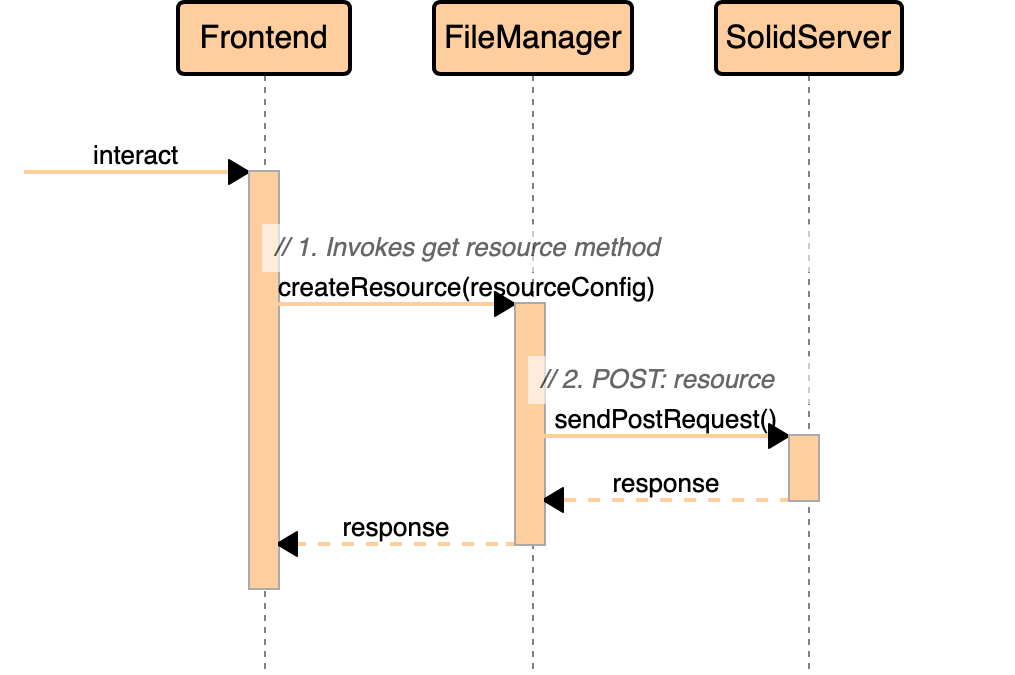
\includegraphics[width=8cm]{lpas_create_resource.png}
\caption{Sequence diagram for POST resource operation invoked from StorageFileManager.}
\label{fig:lpas_create_resource}
\end{figure}

\subsubsection{Reading resources}

Reading the resources demonstrated on figure \ref{fig:lps_get_resource_sequence} is a straightforward set of interactions with an \solid{} specification compliant server, and it can be described as follows:

\begin{enumerate}
    \item \lpa{} frontend invokes the FileManager abstraction with a request specified in \texttt{ResourceConfig} abstraction. The configuration provided contains information on the type of the resource, whether it is a folder or a file, as well as all required information to identify the resource within the POD.
    \item \lpas{} constructs an HTTP GET request to obtain the information from \solid{} server from the provider, the response is forwarded asynchronously.
\end{enumerate}


As demonstrated in the steps above, the LDP specification provides advantages by narrowing down the amount of resource lifecycle related calls as a set of elementary CRUD operations. Another important detail is that every single resource created by \lpas{} is an RDF file. We will cover more information and demonstrate why it is implemented in that way in the proceeding chapter.  
 
\begin{figure}[h]
\centering
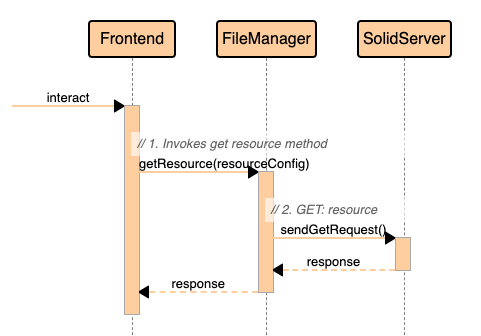
\includegraphics[width=8cm]{get_resource.png}
\caption{Sequence diagram for GET resource operation invoked from StorageFileManager.}
\label{fig:lps_get_resource_sequence}
\end{figure}

\subsubsection{Renaming resources}
\label{ssssec:renaming_resources}

The rename operation covers one of the functional requirements on the \lpa{} platform. It is based on a simpler CRUD operations such as \textit{create} and \textit{read} resource described in earlier sections. The goal of this function is to provide the ability for a \lpa{} developer to implement a functionality to let \lpa{} platform users to choose and manipulate their storage configuration folders.

The flow in the sequence diagram displayed in figure \ref{fig:lps_rename_resource} consists of the following steps:

\begin{enumerate}
    \item \lpa{} frontend invokes the FileManager abstraction with a request specified in the \texttt{ResourceConfig} abstraction, which is similar to the input steps in the previous sequence diagrams. 
    \item \lpas{} has a conditional check to see whether the new provided resource configuration is not accidentally the resource under the same title. This step is followed if the new path and title for a configuration are not equal to an old configuration.
        \begin{enumerate}
        \item Invoke the copy method that will depend on the resource either will copy it directly, if it is a file, or copy it recursively if it is a folder. For the sake of reducing the unnecessary details, the internals of the copy resource call is not displayed on this diagram.
        \item After copying the content of configuration into a new destination, the old resource is removed using the delete operation.
        \end{enumerate}
    \item \lpas{} returns a successful promise since no renaming is invoked in that case. 
\end{enumerate}

\begin{figure}[h]
\centering
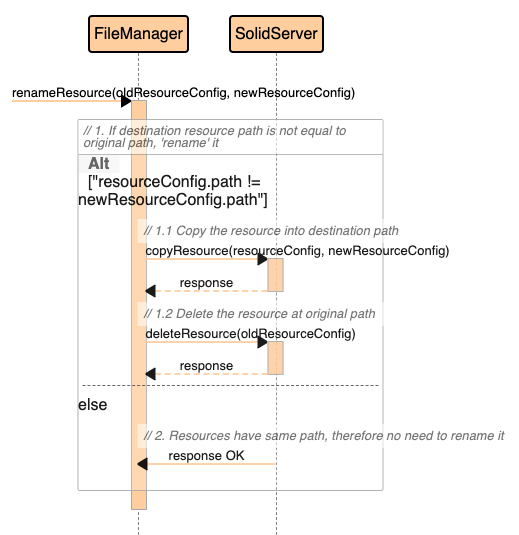
\includegraphics[width=10cm]{rename_resource.png}
\caption{Sequence diagram for a complex operation to rename a particular resource in StorageFileManager.}
\label{fig:lps_rename_resource}
\end{figure}

\subsubsection{Deleting resources}

The deletion of resources is slightly more complicated in comparison with the trivial GET, POST, PUT, and PATCH operations described in earlier sections. The main goal here is to differentiate the type of the resource, and depending on whether it is an LDP Basic Container or generic LDP Resource, act accordingly to delete all files under that resource. 
The flow from figure \ref{fig:lps_delete_resource} can be described as follows:

\begin{enumerate}
    \item Similar to the previous sequence flows, the action is triggered by an input request from \lpa{} frontend
    \item If the resource is and LDP Resource, FileManager trivially sends 
       a single DELETE request to the server and returns the response
    \item If the resource is an LDP Basic Container:
        \begin{enumerate}
        \item Invokes a method for recursively deleting the contents of a folder.
        \item Within that method, it performs a call that fetches the raw RDF describing the LDP Basic Container and parses the resources contained within using. 
        \item Iterate over files, remove them individually as in the first step.
        \item Iterate over folders, remove them individually as in the first step 
        \end{enumerate}
\end{enumerate}


\begin{figure}[h]
\centering
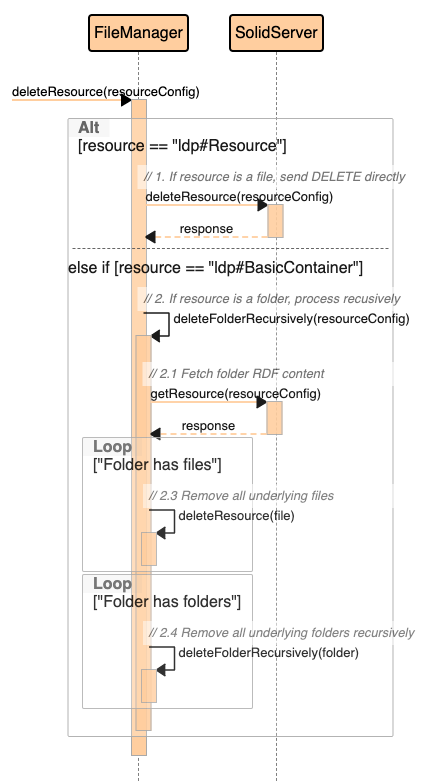
\includegraphics[width=8cm]{delete_resource.png}
\caption{Sequence diagram for a complex operation to delete a particular resource in StorageFileManager.}
\label{fig:lps_delete_resource}
\end{figure}


One of the assumptions made in this recursive operation is the interactions with ACL files when a recursive delete is performed. As mentioned in the introduction to this chapter, \solid{} community is still at its beginnings, and there are many significant improvements yet to introduce. In order to make the delete operation more generic, the DELETE interactions with ACL files had to be removed due to a more strict access policy established between providers of the server and \solid{} apps. The following section will dive deeper into Access Control Managements and related functionality.

\subsubsection{Classes overview}

File manager is the biggest of all three abstractions displayed on the figure \ref{fig:lpas_high_level_abstractions}. Therefore, in order to better describe the architecture of it, a more detail class diagram is provided on figure \ref{fig:lps_file_manager_class_uml}.

\begin{itemize}
	\item The core class available to \lpa{} developers is the \textit{StorageFileManager}. All of the functions inside are intended to be public, static and asynchronous. 
	\item \textit{ResourceConfiguration} is a wrapper for LDP Containers and LDP Resources. It allows a developer to specify \textit{title}, \textit{path} and \textit{type} of a resource. Most of the operations within the \textit{StorageFileManager} are operated with the resources encapsulated into \textit{ResourceConfiguration} classes. It also provides a few helper getters that allow to generate an absolute path to a resource within a pod. 
	\item The \textit{AccessControlConfig} is a subclass of \textit{ResourceConfig}. It allows to specify the access control modes to individual resources. Additionally, it introduces a few extra functions to generate the absolute path that includes the ACL file extension.   
	\item The \textit{SolidResource} is a simple interface that includes various details specific to the resource. Some of the fields provided are also directly used by \textit{StorageFileManager} abstraction during construction of CRUD calls to \solid{} providers.
\end{itemize}


\begin{figure}[h]
\centering
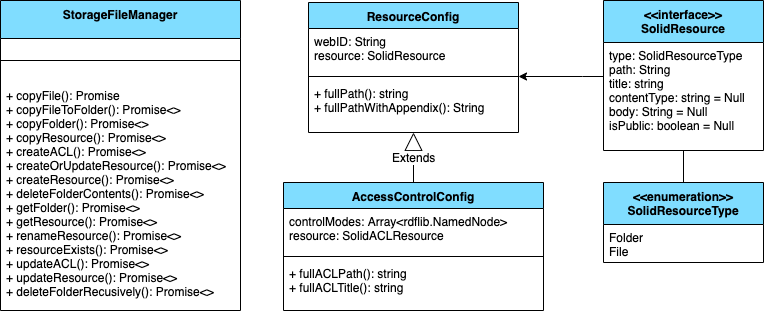
\includegraphics[width=14cm]{lpas_storage_file_manager_uml.png}
\caption{A higher level class diagram of classes contained within StorageFileManager abstraction.}
\label{fig:lps_file_manager_class_uml}
\end{figure}


\subsection{Access Control Manager}
\label{sssec:access_control_manager_arch}

The primary responsibility of the Access Control Manager is a subset under File Manager abstraction. It is designed to support the File Manager entities and provide an ability to wrap them with Web Access Control compliant settings. In other words, this allows a developer of \lpa{} to programmatically control the Read and Write access to any resource inside an arbitrary \solid{} POD by utilizing the developer-friendly interfaces and classes defined within the scope of this abstraction. Essentially, every ACL file is nothing more than yet another RDF resource with few extra features. Hence, the abstraction was placed under the File Manager since the core logic is concerned with similar resource lifecycle manipulations.

It is yet another wrapper on top of the functionality provided by any \solid{} compliant servers. In this case, being \solid{} compliant also assumes conforming to Web Access Control or WAC specification. It defines the so-called Access Control Resources, which are entities serving as the declaration of access control privileges for a specific resource. Within the context of \solid{} specification this means managing access rights to resources in \solid{} PODS for various WebIDs.

The main function provided by the abstraction is an ACL file generator. The flow on the figure \ref{fig:lps_acl_update_flow} demonstrated the process of generation, parsing, and serialization of ACL files: 

\begin{enumerate}
    \item Create Access Control triples for specified input resource configuration files.
    \item Create individual triples defining ACL configuration for a resource owner.
    \item Create individual triples for public access if the resource itself is marked as public.
    \item Gather and parse those triples into a rdflib abstraction representing an RDF Graph.
    \item Serialize this graph instance into a string representing a TTL file.
    \item Finally performs an HTTP call, that uses PUT to create an ACL file attached to a specified resource.
\end{enumerate}

This concludes the section demonstrating the essential abstractions within the \lpas{} package. The consecutive chapters dedicated to Documentation will cover and provide more details regarding less significant classes and utilities available inside the package.

\begin{figure}[h]
\centering
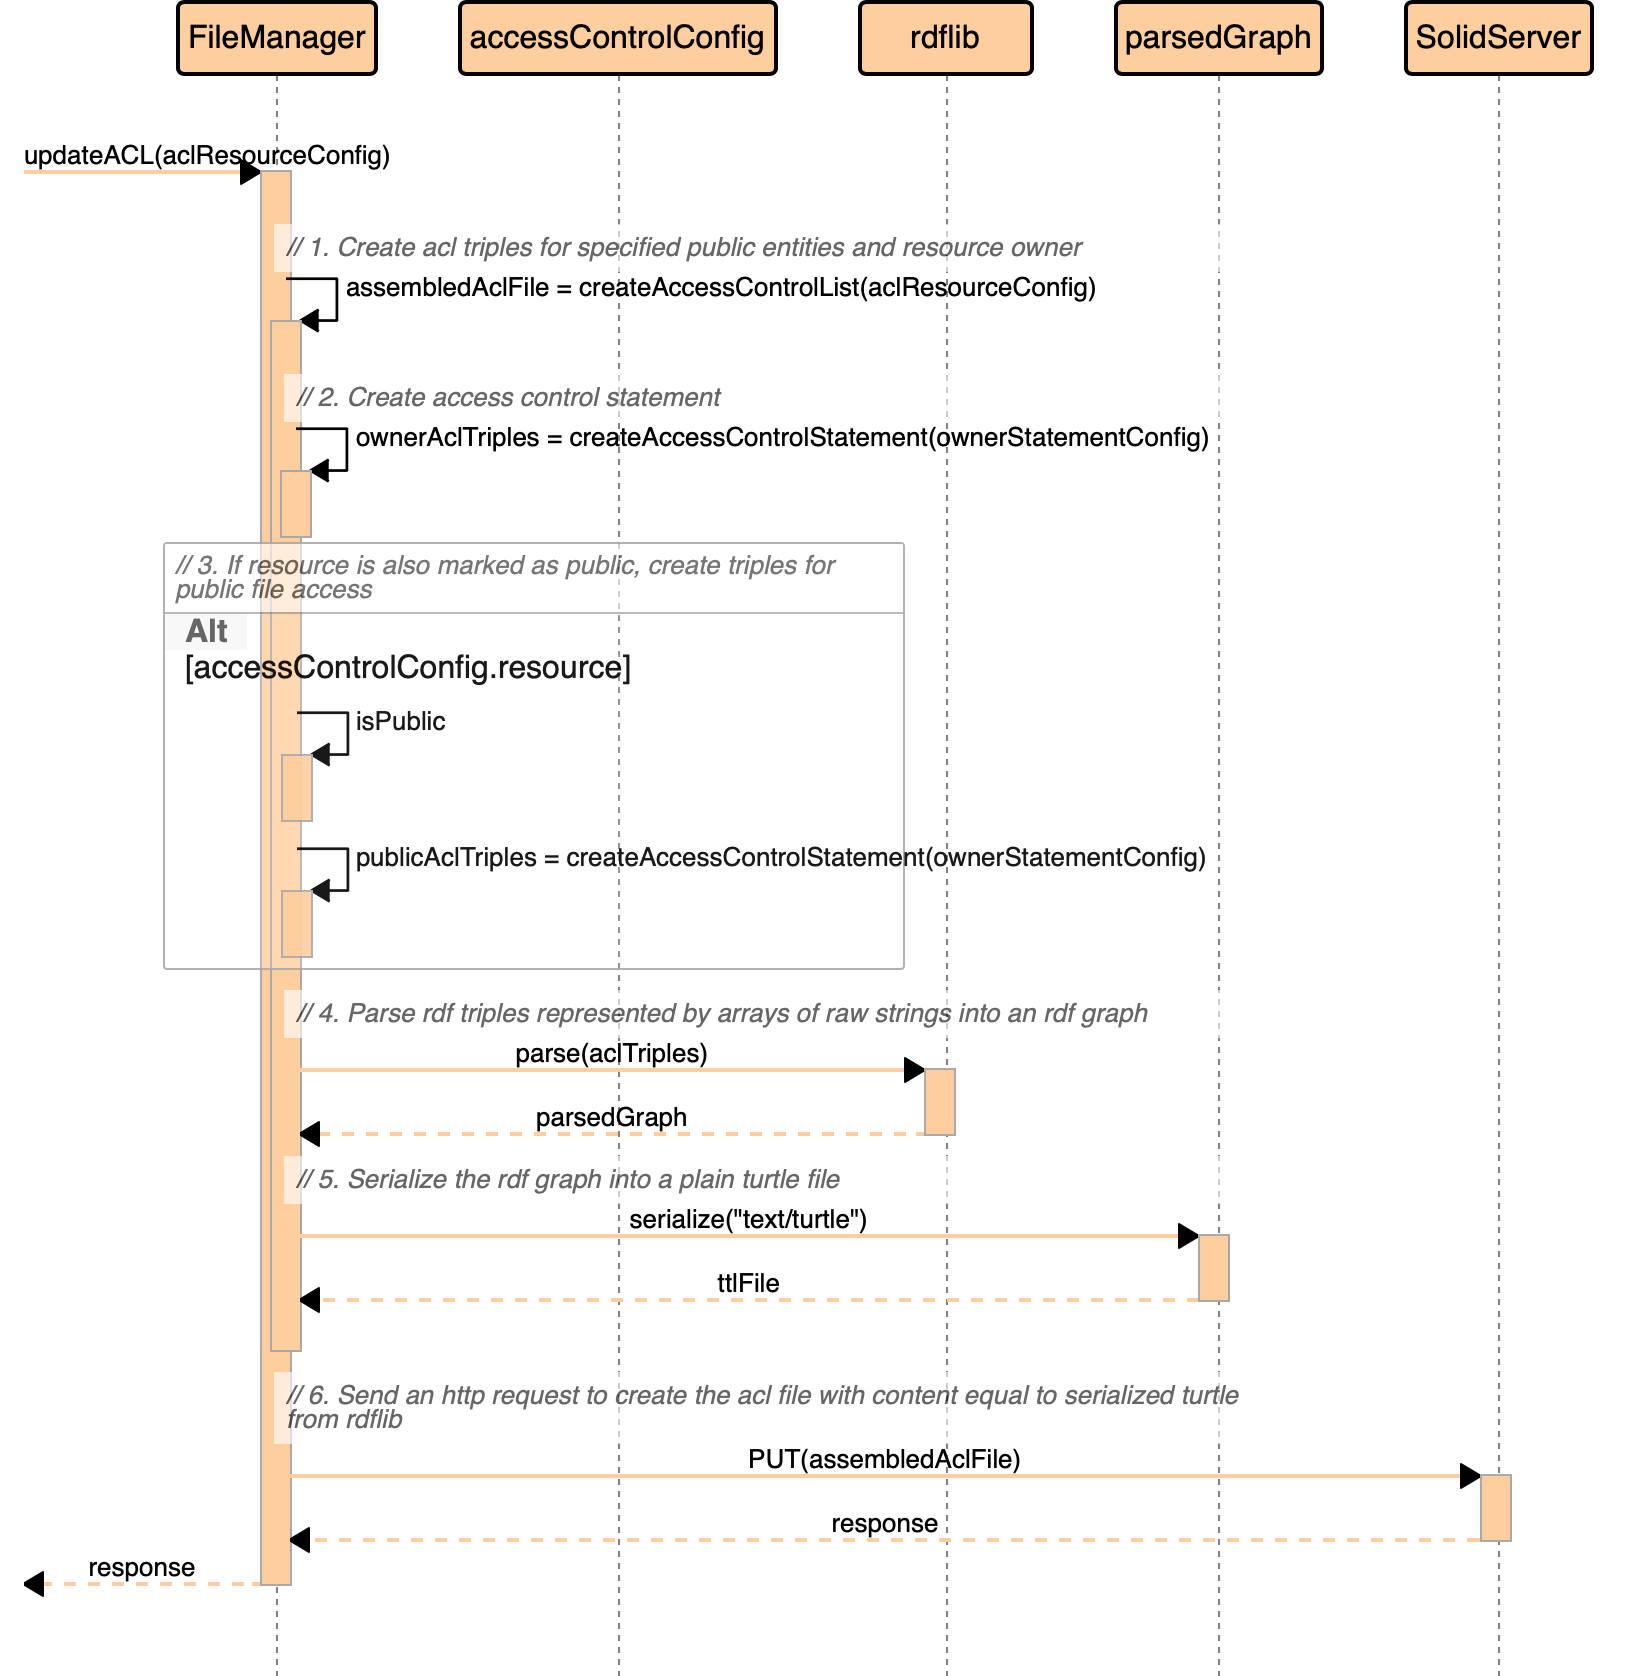
\includegraphics[width=14cm]{acl_update_flow.png}
\caption{A higher level class diagram of classes contained within StorageFileManager abstraction.}
\label{fig:lps_acl_update_flow}
\end{figure}


\section{LinkedPipes Applications Ontology}
\label{ssec:lpas_application_ontology_arch}

Relying on LDP specification extended by \solid{} was not the only goal while designing an architecture to satisfy the requirements of \lpa{}. It was also essential to use the advantages of Linked Data in general. As stated in introductory chapters, as well as the original paper \TODO{cite}, one of the significant benefits of any \solid{} compliant server is that everything is either an RDF file or has the metadata expressed as an RDF file \cite{solid_original_paper}\cite{solid_demo_paper}.  

The first task was to identify and analyze the kind of data \lpa{} is storing. The initial implementation on \lpa{} codebase was a simple application configuration JavaScript object that assembles all required configuration information for an application by the time a user of \lpa{} hits the \textit{Publish} button. In other words, we were given a JavaScript object to operate. Let us describe how this input requirement was taken into consideration while designing a solution that is both optimized for \solid{} and satisfies the requirement. 


\subsection{Using Web Ontology Language}
\label{sssec:using_web_ontology_language}

The Web Ontology Language or OWL, is a commonly used knowledge representation language used for:
\begin{itemize}
	\item Designing ontologies.
	\item Formalizing domains.
	\item Defining domain specific classes and properties.
\end{itemize}

As a first step, the JavaScript object that was used to represent \lpa{} configurations was formalized into a JSON Schema \footnote{\url{https://json-schema.org}}. Based on that Schema, the initial OWL ontology was designed using Stanford Protege \footnote{\url{https://protege.stanford.edu}}, which is a convenient open-source ontology editing tool. The class hierarchy on \autoref{fig:lpas_vocabulary_visualization} demonstrates the draft of the ontology created based on that Schema.

\begin{figure}[h]
\centering
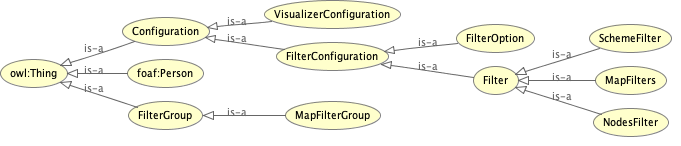
\includegraphics[width=14cm]{lpas_vocabulary_visualization.png}
\caption{A class hierarchy visualization of \lpa{} vocabulary.}
\label{fig:lpas_vocabulary_visualization}
\end{figure}

\subsubsection{foaf:Person}

The \textit{foaf:Person} node on \autoref{fig:lpas_vocabulary_visualization} refers to a WebID profile of an author of this configuration. Due to the generality of the WebID, there was no need to make a specific subclass from the foaf:Person class for that use-case.

\subsubsection{Configuration}
\label{ssssec:configuration}

The \textit{Configuration} class is the main generic abstraction for all \lpa{} configurations. Class hold the generic object properties that can be described as follows:
\begin{itemize}
	\item \textit{author}, this refers to the foaf:Person class stated before, and identifies the person with his WebID as an author of this \lpa{} configuration.
	\item \textit{published}, a date timestamp used to identify when configuration was created and published.
	\item \textit{title}, represents the title given to that \lpa{} visualizer.
\end{itemize}

The class is also a parent class for two subclasses titled \textit{VisualizerConfiguration} and \textit{FilterConfiguration}. More details on them provided in the implementation chapter. However, at this point, it is sufficient to understand that there are two main configuration types. One of them tied to the visualization, and the other is to filters that allow filtering information displayed on visualizers.

\subsubsection{FilterGroup}

The \textit{FilterGroup} class is closely related to Filter and FilterConfiguration and is used to reference the aggregation of visualizer specific filters. Since it does not necessarily need to inherit the object properties of FilterConfiguration, it is inheriting from generic \textit{owl:Thing} class.

\begin{figure}[h]
\centering
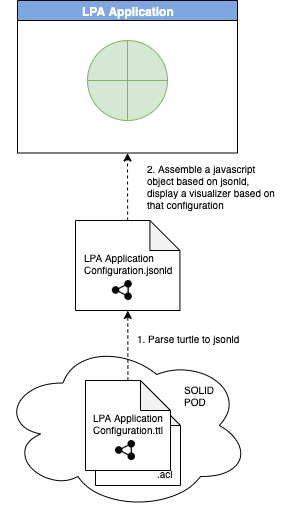
\includegraphics[width=6cm]{lpas_vocabulary_usage.png}
\caption{A formal representation of \lpa{} configurations expressed as RDF files using the \lpas{} vocabulary.}
\label{fig:lpas_vocabulary_usage}
\end{figure}

In order to simplify adoption of this ontology in \lpa{} frontend, the resulting ontology was converted into a JSON-LD Schema \footnote{\url{https://json-ld.org}}, as shown on \autoref{fig:lpas_vocabulary_usage}. However, due to some limitations in NSS, the individual \texttt{jsonld} configurations had to be converted into TTL files when stored in \solid{}. For more details on adoption and  implementation of this ontology refer to \autoref{chap:num_5}.


\section{Storage Component Design}
\label{ssec:lpas_storage_component_design}

It is important to note that the \lpas{} is not just the external package completely isolated from the \lpa{} frontend, it is also a set of React components that attempt to blend in into the user interface guidelines of the frontend. Now when the major components of the \lpas{} package as well as the \lpas{} vocabulary are described, let us dive deeper into the design considerations done on the frontend side inside the \lpa{} codebase. 

The \lpa{} frontend codebase was implemented using React\footnote{\url{https://reactjs.org}} and was utilising a modern stack of frontend development tools, all of those had to be taken into consideration to design React Component responsible for interactions with the storage. This section will cover the design conventions inherited from \lpa{} as well as a detailed overview of User Interfaces conforming to Material Design\footnote{\url{https://material.io/design}} conventions that were strongly utilized in \lpa{} frontend. In addition to that, it will also revisit the functional requirements and provide UI design proposals that are later implemented in the implementation section.

\subsection{Designing React Components}

At the root, \lpa{} frontend identifies two main types of components that are logically separated into folders titled as follows:
\begin{itemize}
	\item \texttt{Components} folder, these usually contain elements that are used in more than one webpage throughout the project, such as buttons, switches, image wrappers and etc.
	\item \texttt{Containers} folder, represent complex react components that are basically rendering individual webpages or sub-elements of webpages that deal with complex user interaction scenarios.
\end{itemize}

\subsubsection{Simple components}

Whenever an individual component needs to be implemented and it will be used in multiple webpages throughout the project, it is being placed into \texttt{Components} folder.

There are two main types of components that can be placed into \texttt{Components} folder and have different design conventions:
\begin{itemize}
	\item Simple stateless component responsible for plain rendering.
	\item A complex component that needs to aggregate multiple sub-components, manage external state, internal states and etc.
\end{itemize}


This is not a strict guideline defined by \lpa{} developers. However, if a component becomes too complex, as demonstrated on figure \ref{fig:lpas_component_design} the intent is to split component into separate component responsible for rendering and component that manages states of the stateless component. This allows easier navigation within frontend codebase as well as faster code debugging. 

\begin{figure}[h]
\centering
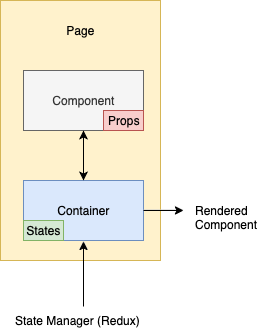
\includegraphics[width=7cm]{lpas_component_design.png}
\caption{React container abstraction decomposition following \lpas{} design conventions.}
\label{fig:lpas_component_design}
\end{figure}

Therefore, the logical decomposition of components by their complexity is the concludes the only major design convention that was required by \lpa{} frontend. Let us go over the details of each individual component in the following sections.

\subsection{Authentication View}
\label{sssec:architecture_auth_view}

Authentication is the entry for the \lpa{} platform, and \lpas{} covers the design and implementation of that view since \lpa{} relies on \solid{} to perform the WebID authentication. 

As previously demonstrated in \autoref{sssec:authentication_manager}, the \lpas{} package handles the authentication by redirecting the requests and responses between the browser of the user and the \solid{} provider server. The mock user interface on \autoref{fig:lpas_authenticate_mock} demonstrates a basic mock for a authentication webpage. There are several ways to authentication available to a \lpa{} user with a WebID profile in any \solid provider:
\begin{itemize}
    \item \textit{Provider authentication}, user clicks on a dropdown pane and selects the name of the default providers. The default providers supported by \lpas{} are \textit{inrupt.net} \footnote{\url{https://inrupt.net}} , \textit{solid.community} \footnote{\url{https://solid.community}} and a self-hosted LinkedPipes server available at \textit{lpapps.co:8443} \footnote{\url{https://lpapps.co:8443}}.
    \item \textit{WebID authentication}, similar to previous option but instead user is able to provide his WebID and be redirected right into the login page of his provider.
\end{itemize} 

\begin{figure}[h]
\centering
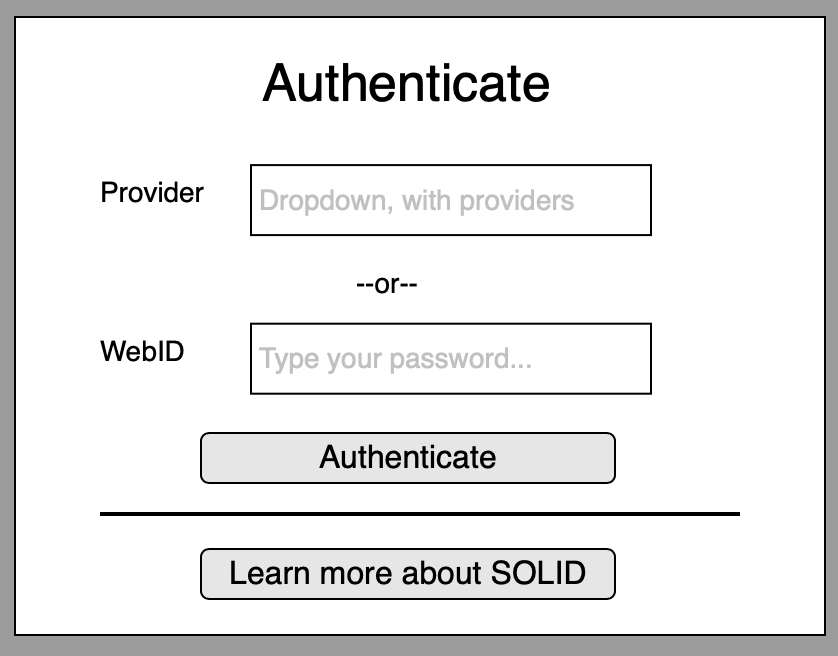
\includegraphics[width=7cm]{lpas_authenticate_mock.png}
\caption{Mock UI for Authentication webpage in \lpa{} Frontend.}
\label{fig:lpas_authenticate_mock}
\end{figure}

The additional user interface elements are defined as follows:

\begin{itemize}
    \item \textit{Authenticate} button executes the authentication sequence depending on the options that users have chosen, which are either Provider or direct WebID authentication.
    \item \textit{Lean more about \solid{}} redirects users not familiar with concepts of \solid{} directly into the home page of the inrupt project.
\end{itemize}
 

\subsection{Storage Dashboard}
\label{sssec:architecture_storage_dashboard}

Referring back to the functional requirements stated in the first chapters, the ability to interact with the \lpas{} is an essential feature allowing users of \lpa{} platform to manipulate their Applications. The mock displayed on \ref{fig:lpas_ui_dashboard_mock} is a webpage accessible via the home dashboard. There are two main display modes:

\begin{itemize}
    \item The \textit{My apps} tab, is a React component that fetches all RDF resources in root \lpas{} folder containing applications created by a user. 
    \item The \textit{Shared} tab is a React component fetching all RDF resources in a shared \lpas{} folder containing applications created and shared by a particular user with other users of \lpas{} platform.
\end{itemize}


\begin{figure}[h]
\centering
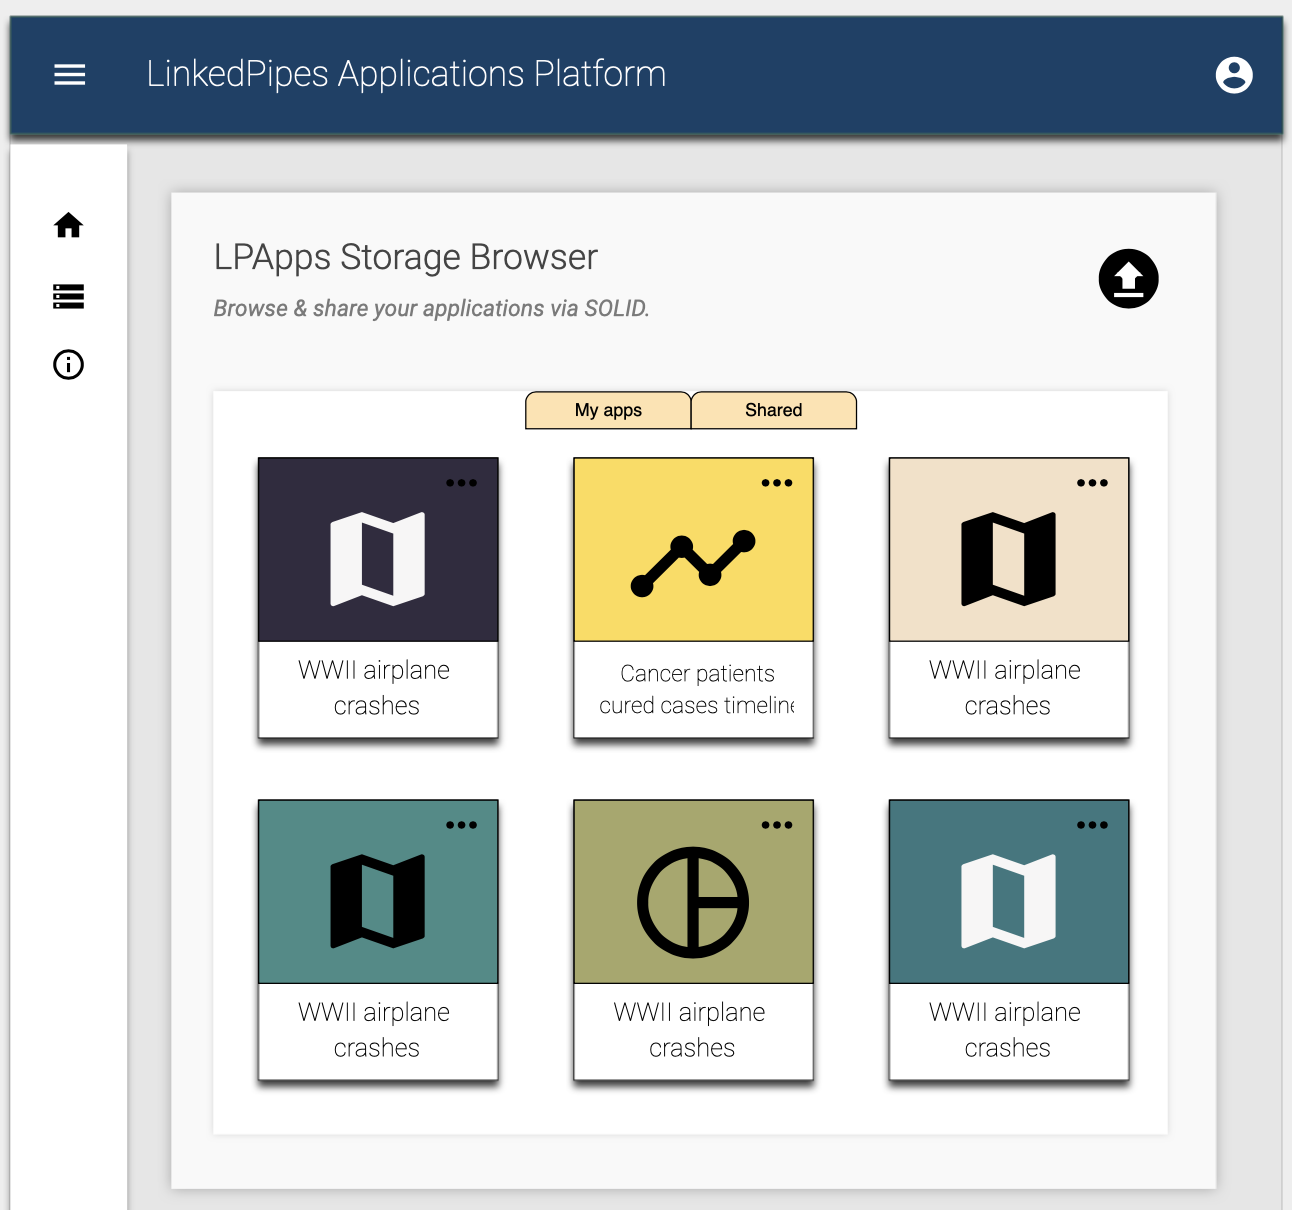
\includegraphics[width=7cm]{lpas_ui_dashboard_mock.png}
\caption{Mock UI for Storage Dashboard webpage in \lpa{} Frontend.}
\label{fig:lpas_ui_dashboard_mock}
\end{figure}



The idea behind the dashboard is that each card is a visual representation of \lpa{} configuration. As mentioned earlier in \autoref{sssec:using_web_ontology_language}, each configuration is expressed using the \lpas{} ontology and stored as an RDF file inside \solid{}. The card collection view pulls each of the configurations from the container, storing them in \solid{} and populates the content. 

The user of \lpa{} has a set of straightforward interactions that can be performed on card:
\begin{itemize}
    \item \textit{Clicking on card}, redirects the user to the webpage displaying the visualizer.
    \item \textit{Clicking on sub-menu icon}, reveals a popup where users can choose to delete, rename, or share the visualizer.
\end{itemize}


\subsection{Storage Control Panel}
\label{sssec:architecture_storage_control_panel}

An ability to authenticate, create, and publish an application using \solid{} are essential requirements stated by \lpa{}. However, users also need to have basic functionality to manipulate the data stored by the \lpas{} within their PODs. Therefore a mock design demonstrated on \autoref{fig:lpas_change_folder_mock} provides the basic functionality described as follows:

\begin{itemize}
    \item \texttt{Update} folder, allows users to switch their root folder into any other folder within their POD.
    \item \texttt{Copy} folder allows users to copy all content from the current root configurations folder into a new or existing folder.
    \item \texttt{Move} folder allows users to move all content from the current root configurations folder into a new or existing folder.
\end{itemize}


\begin{figure}[h]
\centering
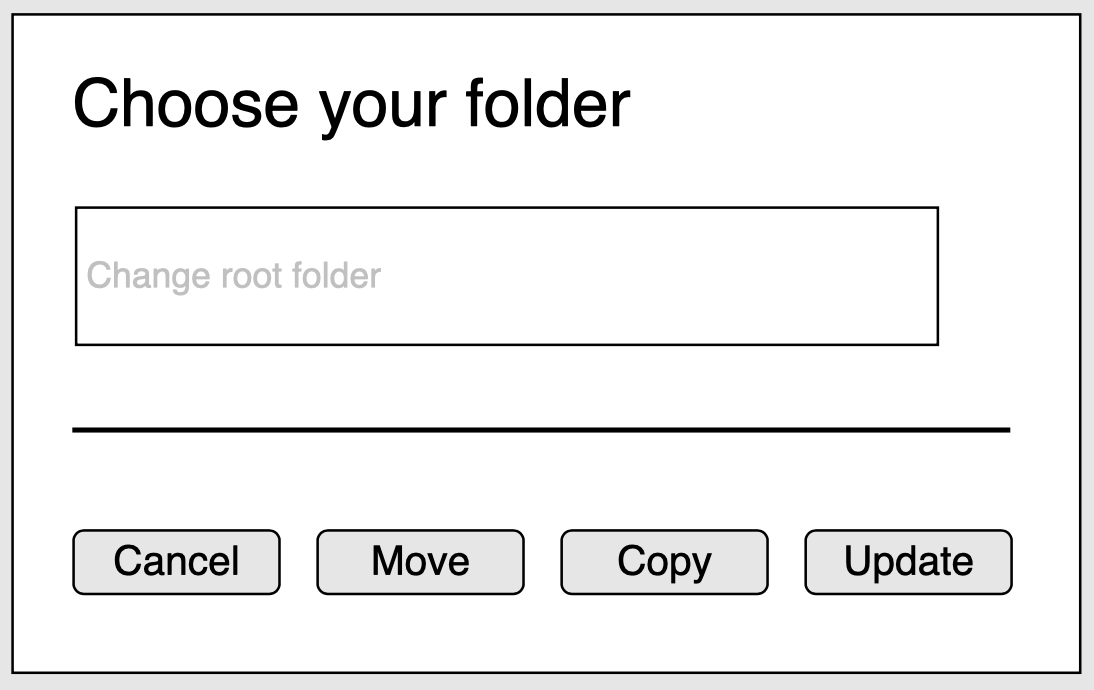
\includegraphics[width=6cm]{lpas_change_folder_mock.png}
\caption{Mock UI for Storage Dashboard webpage in \lpa{} Frontend.}
\label{fig:lpas_change_folder_mock}
\end{figure}

The diagrams in \autoref{ssec:storage} demonstrate the exact sequence of interactions between \lpa{}, \lpas{} and \solid{} providers when operations like \textit{move} or \textit{copy} folder are invoked.

To sum up, this chapter provided an overview of three major aspects of \lpas:
\begin{itemize}
    \item The npm package contains the core abstractions architectured to be separated from the \lpa{} with the intent to improve \solid{} related code maintainability and testing. The sequence diagrams of all main CRUD operations performed on RDF resources in \solid{} PODs.
    \item The \lpas{} ontology, an RDF vocabulary designed specifically for \lpa{} configurations, taking full advantage of \solid{}. In other words, giving an ability not simply to store the \lpa{} configurations, but also perform any complex querying on them using SPARQL.
    \item The frontend React components, the UI mocks of components inside \lpa{} frontend, conforming to conventions of the \lpa{}.
\end{itemize}
In the next chapter, a detailed review of the implementation of the architecture will be provided.




\chapter*{Conclusion}
\addcontentsline{toc}{chapter}{Conclusion}

To summarize, in the following work implements a multipart decentralized storage solution for \lpa{} platform based on \solid{} project. The term multipart reffers to implementation of the \lpas{} npm package, the \lpas{} Ontology used to represent \lpa{} visualizer configurations as RDF files and lastly, a set of Storage Components implemented in \lpa{} frontend. 

An overview of related tools in \autoref{chap:num_2} provided a set of software technologies alternative to \solid{}. The chapter also provided a comparison table described in \autoref{sssec:lpa_preliminaries_component_overview} that demonstrated benefits of choosing \solid{} as a core storage technology for \lpa{} platform.

An analysis and description of \lpa{} requirements and \solid{} development toolset in \autoref{chap:num_3} defined the main practical tasks to be achieved by \lpas{} as well as to which \solid{} libraries and frameworks to utilize in implementatioin. The final reasoning expanding the conclusion from \autoref{chap:num_2} on choosing solid was provided at the end of the chapter in \autoref{sssec:why_solid}.

Based on the performed analysis on \solid{} and requirements stated by \lpa{}, \autoref{chap:num_4} described a detailed overview of a designed architecture of \lpas{}. The architecture consisted of three main parts. Firstly, the \autoref{ssec:storage}, provided the design of abstractions for a \lpas{} npm package providing functionality for authenticating (\autoref{sssec:authentication_manager}), operating the resources inside \solid{} PODs (\autoref{sssec:file_manager}) and managing ACL files (\autoref{sssec:access_control_manager_arch}). Afterwards, the \autoref{ssec:lpas_application_ontology_arch} provided an overview of designed OWL Ontology for representing the \lpa{} visualizer configurations as RDF resources inside \solid{} POD as well as describing the benefits of such approach to storing visualizer data. And lastly, \autoref{ssec:lpas_storage_component_design} provided a set of designed user interface mocks complying to stated \lpa{} requirements as well as a detailed overview of the functioinality provided by those user interface components.

Continuing the architecture overview, \autoref{chap:num_5} described the entire implementation of the storage functionality and structured similar to the previous chapter as it implements the designed elements in order with their design and architecture. The \autoref{ssec_storage_package_implementation} provided detailed overview of the \lpas{} package implementation using TypeScript programming language. The \autoref{ssec:storage_ontology_implementation} described the process of implementing and hosting the designed \lpas{} Ontology using Protégé and Ontology open-source tools. The \autoref{sssec:lpas_storage_frontend_implementation} described the implementation of Storage React components inside the \lpa{} frontend codebase. The final renders of components were demonstrated in \autoref{ssec:overview_of_implemented_requirements} by iterating of functional requirements. Lastly, in \autoref{ssec:non_functional_requirements_implementation} an overview of implemented non-functional requirements was provided. Chapter also clearly demonstrated that all defined functional and non-functional requirements of \lpa{} were covered and implemented, thus fulfilling the practical goals of the thesis.

The \autoref{chap:num_6} demonstrated the improvements introduces to \lpa{} after evaluating the platform with fully integrated \lpas{} solution. The chapter also provided the main results and achievements obtained as a part of the implementation stage and evaluation process, such as:
\begin{itemize}
    \item Recognition on official website of the \solid{} project (\autoref{sssec:recogniition_on_solid}).
    \item Comments and short conversations with Sir Tim Berners-Lee in regards to questions on \solid{} specifications asked by author (\autoref{sssec:comments_from_tim}).
    \item Demonstration of user traction over a six month period of continious delivery of the \lpas{} solution. Positive feedback and recognition by \solid{} community members and member of BARTOC organization (\autoref{sssec:user_traction_of_platform}).  
\end{itemize}
 
A detailed overview of the testing of \lpas{} solution was provided in \autoref{chap:num_7}. In \autoref{ssec:lpas_unit_testing} a demonstration of how the \lpas{} package itself was unit tested and automated with Continious Integration and Delivery pipelines using Travis CI. And lastly, in \autoref{ssec:integration_and_delivery} an overview of improvements introduced into \lpa{} automated build pipelines and integration testing of both \lpa{} and \lpas{} solutions was provided.

The whole \lpas{} solution was thoroughly documented both on the npm package side as well as by expanding the \lpa{} documentation to include Storage Components as described in \autoref{chap:num_8}.

\section{Future work}

The \solid{} ecosystem is constantly expanding in its specifications, community, and available technological toolset. Throughout fulfilling the goals of the thesis, many challenges were faced due to the aforementioned constant changes in the \solid{} project. Over time once, \solid{} technology will mature for more advanced production level use cases, and the ecosystem of decentralized social applications will grow. The dependencies such as node-solid-server and solid-auth-client used in \lpas{} package might require significant updates and refactor. Additionally, by the time of finishing the practical part of this thesis, several libraries were introduced by official \solid{} contributors, including a brand new \solid{} server implementation in TypeScript called \texttt{pod-server} \footnote{\url{https://github.com/inrupt/pod-server}} aimed to eventually replace the node-solid-server. Aside from that a library called \texttt{tripledoc} \footnote{\url{https://vincenttunru.gitlab.io/tripledoc/}} was introduced, aiming to potentially become the standard library to interact and manage resources in \solid{} PODs. 

Therefore, potential improvements and future work in \lpas{} package and storage components include the following:
\begin{itemize}
    \item \textit{Gradual refactoring and replacement of node-solid-server}. Replacing the node-solid-server implementation with more stable and actively supported pod-server implementation could introduce more user-friendly experience while performing authentication and manipulation of resources inside PODs.
    \item \textit{Gradual integration of tripledoc into \lpas{} package}. As tripledoc potentially offers the same functionality as the \lpas{} package, the potential future work includes replacing certain low-level interactions with rdflib and using tripledoc instead. This can simplify the maintainability of \lpas{} package, simplify unit-testing, and can potentially make it a generic utility for storing and managing any configuration ontologies in \solid{}.
    \item \textit{Improving collaborative editing}. One of the extra features implemented within the scope of \lpas{} was the ability to share published applications within users of \lpa{} platform and let them configure the published application collaboratively. An improved version of that can include real-time editing of the resources more robustly, while the current version discards any simultaneous real-time changes submitted by collaborating users.
    \item \textit{General support of the project}. This, of course, assumes the long term general support of the solution and parts of \lpa{} platform covering the Storage functionality to keep it up to date with all the latest improvements and changes introduces in \solid{} specification.
\end{itemize}

The ambitious goal of decentralizing the World Wide Web set by Sir Tim Berners-Lee is yet to demonstrate its benefits and receive a more comprehensive recognition across non-developer oriented domains and average internet users. However, we believe that the fundamental specifications of \solid{} project that improves upon established Web Standards, an active and passionate community, and a developer-friendly environment and tools to builds decentralized social applications will define the next generation of internet technologies and make it more secure and privacy-oriented.

%%% Bibliography
%%% Bibliography (literature used as a source)
%%%
%%% We employ bibTeX to construct the bibliography. It processes
%%% citations in the text (e.g., the \cite{...} macro) and looks up
%%% relevant entries in the bibliography.bib file.
%%%
%%% The \bibliographystyle command selects, which style will be used
%%% for references from the text. The argument in curly brackets is
%%% the name of the corresponding style file (*.bst). Both styles
%%% mentioned in this template are included in LaTeX distributions.

\bibliographystyle{plainnat}    %% Author (year)
% \bibliographystyle{unsrt}     %% [number]

\renewcommand{\bibname}{Bibliography}

%%% Generate the bibliography. Beware that if you cited no works,
%%% the empty list will be omitted completely.

\bibliography{bibliography}

%%% If case you prefer to write the bibliography manually (without bibTeX),
%%% you can use the following. Please follow the ISO 690 standard and
%%% citation conventions of your field of research.

% \begin{thebibliography}{99}
%
% \bibitem{lamport94}
%   {\sc Lamport,} Leslie.
%   \emph{\LaTeX: A Document Preparation System}.
%   2nd edition.
%   Massachusetts: Addison Wesley, 1994.
%   ISBN 0-201-52983-1.
%
% \end{thebibliography}


%%% Figures used in the thesis (consider if this is needed)
\listoffigures

%%% Tables used in the thesis (consider if this is needed)
%%% In mathematical theses, it could be better to move the list of tables to the beginning of the thesis.
\listoftables


%%% Show glossary
% Add to the glossary all the words defined, regardless of whether they are actually referenced in the document or not
\glsaddall
% \printglossaries
% \printnoidxglossary[type=\acronymtype]
\printnoidxglossary[title=Glossary]
\printnoidxglossary[type=acronym]

%%% Attachments to the master thesis, if any. Each attachment must be
%%% referred to at least once from the text of the thesis. Attachments
%%% are numbered.
%%%
%%% The printed version should preferably contain attachments, which can be
%%% read (additional tables and charts, supplementary text, examples of
%%% program output, etc.). The electronic version is more suited for attachments
%%% which will likely be used in an electronic form rather than read (program
%%% source code, data files, interactive charts, etc.). Electronic attachments
%%% should be uploaded to SIS and optionally also included in the thesis on a~CD/DVD.
%%% Allowed file formats are specified in provision of the rector no. 72/2017.
\appendix
\chapter{Attachments}

\section{First Attachment}

\openright
\end{document}
